%%%%%%%%%%%%%%%%%%%%%%%%%%%%%%%%%%%%%%%%%%%%%%%%%%%%%%%%%%%%%%%%%%%%%%%%%%%%%%%%
\documentclass[letterpaper, 10 pt, conference]{ieeeconf}

\IEEEoverridecommandlockouts
\overrideIEEEmargins

\usepackage[UTF8,fontset=none,scheme=plain]{ctex}
\setmainfont{Times New Roman}
\setCJKmainfont{Songti SC}
\setCJKsansfont{PingFang SC}
\setCJKmonofont{Songti SC}
\usepackage{amsmath}
\usepackage{subcaption}
\usepackage{booktabs}
\usepackage{caption}
\usepackage{tabularx}
\usepackage{multirow}
\usepackage{graphicx}
\usepackage{array}
\usepackage[export]{adjustbox}
\usepackage{xcolor}
\usepackage{hyperref}
\usepackage[normalem]{ulem}

\newcommand{\rev}[1]{{\color{black}#1}}
\newcommand{\sys}{\rev{RoboHarness}}
\newcommand{\titleemoji}{%
  \raisebox{-0.18ex}{
\includegraphics[height=1.25em,trim=220 80 150 80,clip]{figure/harness_big_head.png}}%
}
\pdfstringdefDisableCommands{%
  \def\rev#1{#1}%
  \def\sys{RoboHarness}%
  \def\titleemoji{}%
}

\title{\LARGE \bf
\rev{RoboHarness~\titleemoji：通过上下文内自适应提升视觉--语言--动作模型鲁棒性的记忆增强策略外壳}
}

\author{
    \authorblockN{Zhuoran Li$^{1,*}$, Zhiyang Li$^{1,*}$, Kaijun Zhou$^{1}$, Jinyu Gu$^{1,2,\dagger}$} \\
}

\begin{document}

\twocolumn[{
    \renewcommand\twocolumn[1][]{#1}
    \maketitle
    \thispagestyle{empty}

    \vspace{-4em}
    \begin{center}
        \centering
        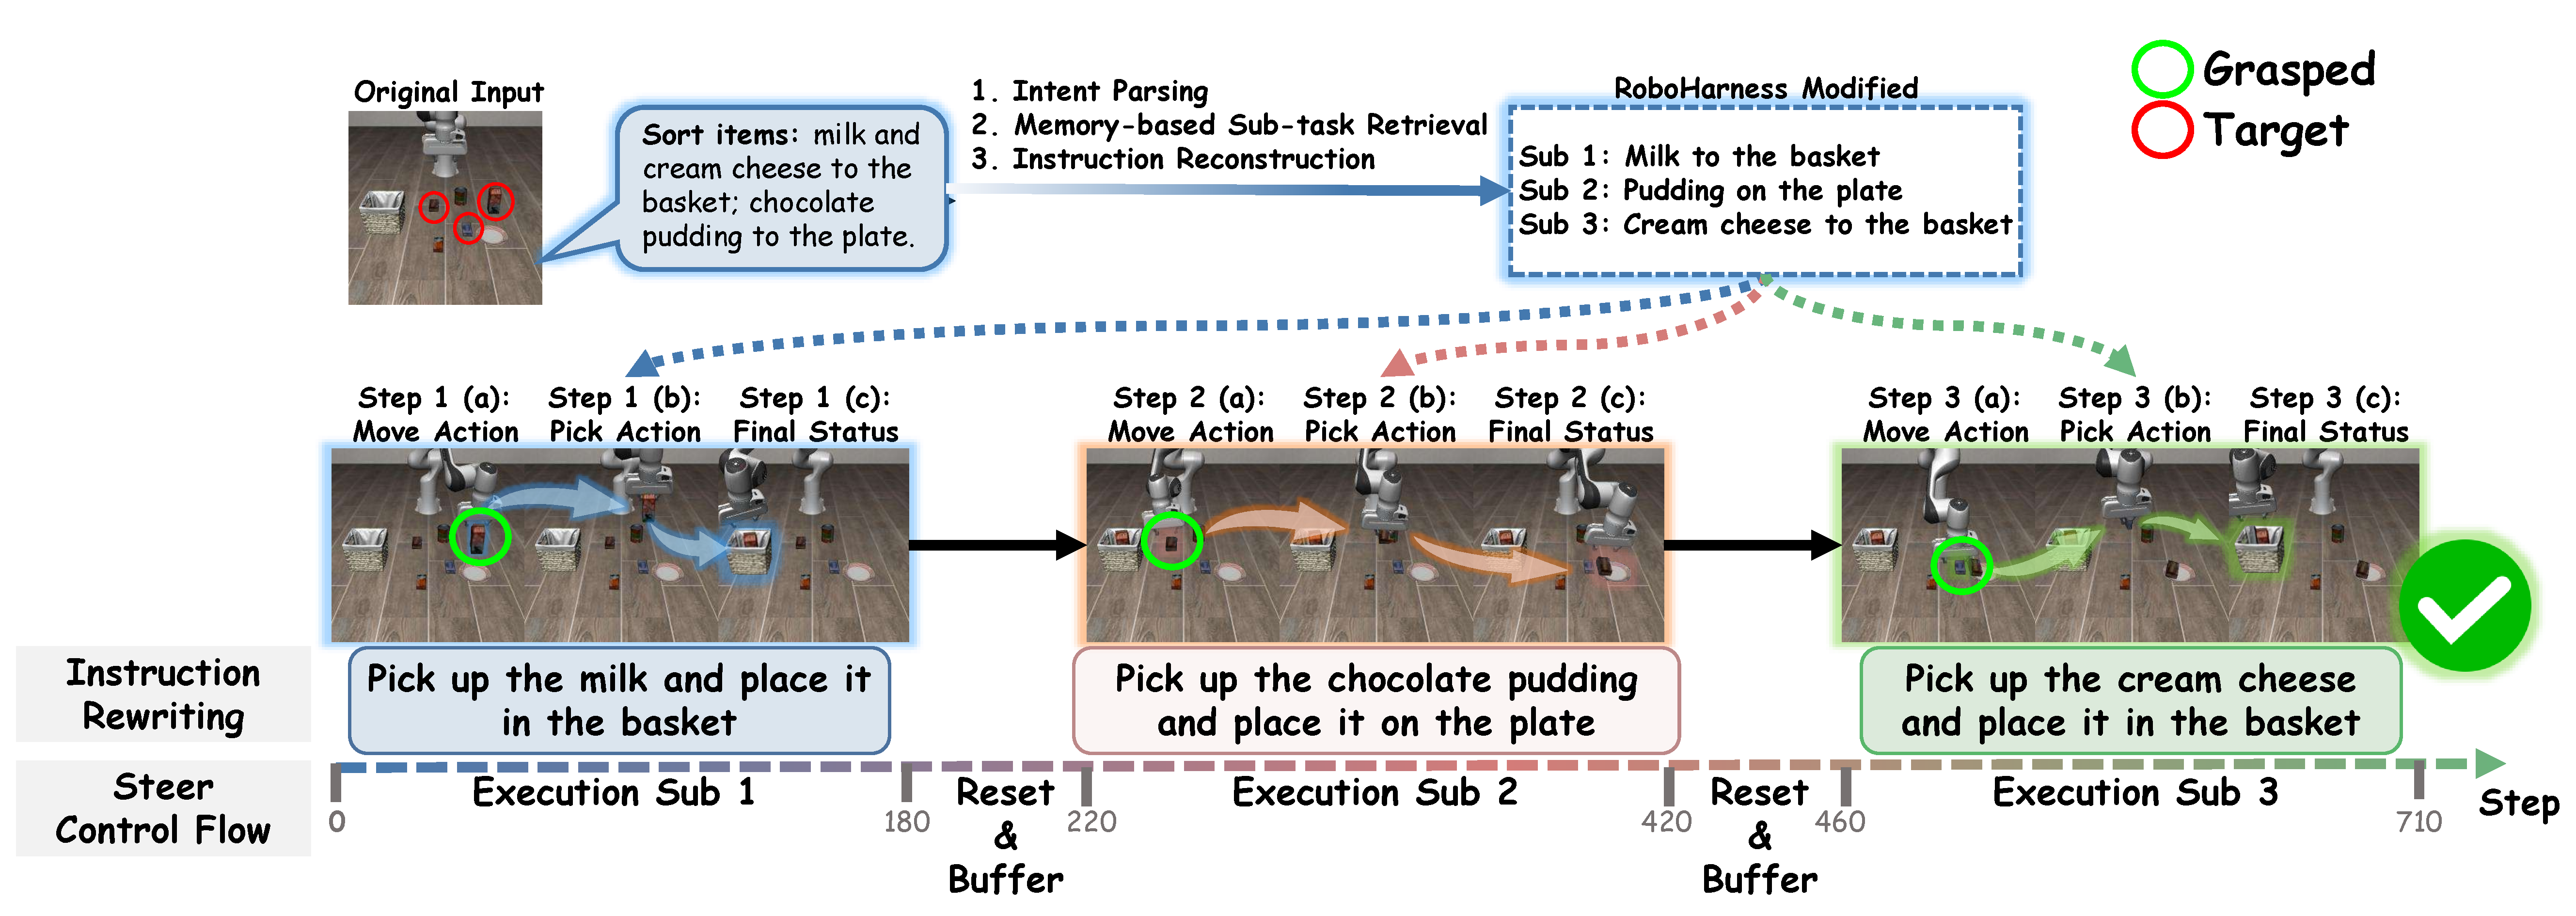
\includegraphics[width=0.95\textwidth]{figure/long_horizon.pdf}
        \captionof{figure}{\textbf{记忆驱动的长时程操作分解。}
        \sys\ 通过意图解析、记忆检索和自适应控制流调节，将抽象的多步指令转换为可执行序列。}
        \label{fig:long_horizon}
    \end{center}
}]

\pagestyle{empty}

\begin{abstract}
尽管视觉--语言--动作（VLA）模型有望成为通用机器人控制器，但由于缺乏长期记忆、因果失败归因和动态干预能力，它们在分布外（OOD）任务中抵御感知噪声与环境变化的鲁棒性仍受到根本限制。
为解决这一问题，我们提出 \sys：一种记忆增强的策略外壳，无需参数微调即可升级冻结的 VLA 策略，实现鲁棒的上下文内自适应。
具体而言，\sys\ 的在线流水线由对比式双记忆检索增强生成（RAG）、基于多模态大语言模型实现的归因驱动视觉--语言编排器，以及可扩展的模型上下文协议（MCP）干预组成；与此同时，离线记忆巩固模块持续将执行轨迹提炼为可靠先验。
我们在 LIBERO-PRO 和新提出的 LIBERO-\sys\ 基准上，使用三个骨干模型（$\pi_0$、$\pi_{0.5}$ 和 SmolVLA）进行实验评估。结果表明，\sys\ 使成功率平均绝对提升 $\mathbf{56.6\%}$，其中长时程任务串联的绝对提升达到 $\mathbf{89.1\%}$。
项目页面和源代码见：\url{https://github.com/LZY-1021/RoboHarness}。
\end{abstract}

\section{引言}
\renewcommand{\thefootnote}{\fnsymbol{footnote}}
\footnotetext[1]{同等贡献。}
\footnotetext[2]{通讯作者：Jinyu Gu {\tt\small <gujinyu@sjtu.edu.cn>}。}

\renewcommand{\thefootnote}{\arabic{footnote}}
\footnotetext[1]{上海交通大学计算机学院，中国上海。}
\footnotetext[2]{上海悉龙信息科技有限公司。}

VLA 模型已成为端到端机器人操作的一种主导范式，它在单一可学习策略中统一多模态感知、语言落地和连续运动控制~\cite{VLA_review1, VLA_review2}。
本文所称的多模态，特指联合使用视觉观测或关键帧与自然语言指令，以完成落地、检索和干预规划，而非任意组合机器人传感器模态。
在部署时，这些模型充当整体式的感知--运动控制器，直接将视觉观测和自然语言指令转换为底层运动命令。

然而，随着机器人智能体从受控实验室走向开放世界环境，核心挑战已从分布内准确性转向鲁棒的上下文内自适应~\cite{Yuan2025FromST}。
微调在专门场景中虽然有效，但通用机器人会面临训练期间无法充分预见的干扰和噪声。
物体外观、光照和语言的变化往往引发 OOD 扰动，暴露出静态 VLA 策略的局限，也说明系统必须能够抵御环境噪声和因果干扰项~\cite{RT-2, hill2020humaninstructionfollowingdeepreinforcement, pmlr-v205-shah23b, liberopro,LIBERO-Plus}。

现有方法只能部分解决 OOD 泛化问题。
以规模扩展为中心的基础模型~\cite{pi0, openvla, openx}试图从大规模数据中获得泛化能力，但仍是无状态控制器：它们会丢弃执行历史，缺少 OOD 自适应所需的\textbf{长期记忆}。
检索增强框架~\cite{ricl, memer}利用以往示范，却受到“成功偏置”的影响：由于只模仿成功轨迹，它们缺少从感知差异中诊断失败的\textbf{因果归因}能力。
这两类范式还都将知识视为静态产物，导致早期错误归因在任务之间持续存在。
近期的智能体框架~\cite{cap, voxposer, moka}加入基于 LLM/VLM 的规划，但仍是从零开始推理，且工具集成僵化，缺少干预感知--动作流所需的\textbf{动态编排}能力。

这些观察表明，要实现鲁棒的 OOD 泛化，需要一个能够有效整合下列能力的统一框架：
\emph{(i)} 用于积累并复用既往执行经验的长期记忆；
\emph{(ii)} 因果归因和失败感知的策略调整；
\emph{(iii)} 对外部工具进行动态编排，以主动干预感知--动作流；以及
\emph{(iv)} 持续改进所存经验、避免知识停滞的自演化巩固机制。

\begin{figure}[t]
\vspace{0.5em}
     \centering
     \captionsetup[subfigure]{font=footnotesize}
     \begin{subfigure}[b]{0.15\textwidth}
         \centering
         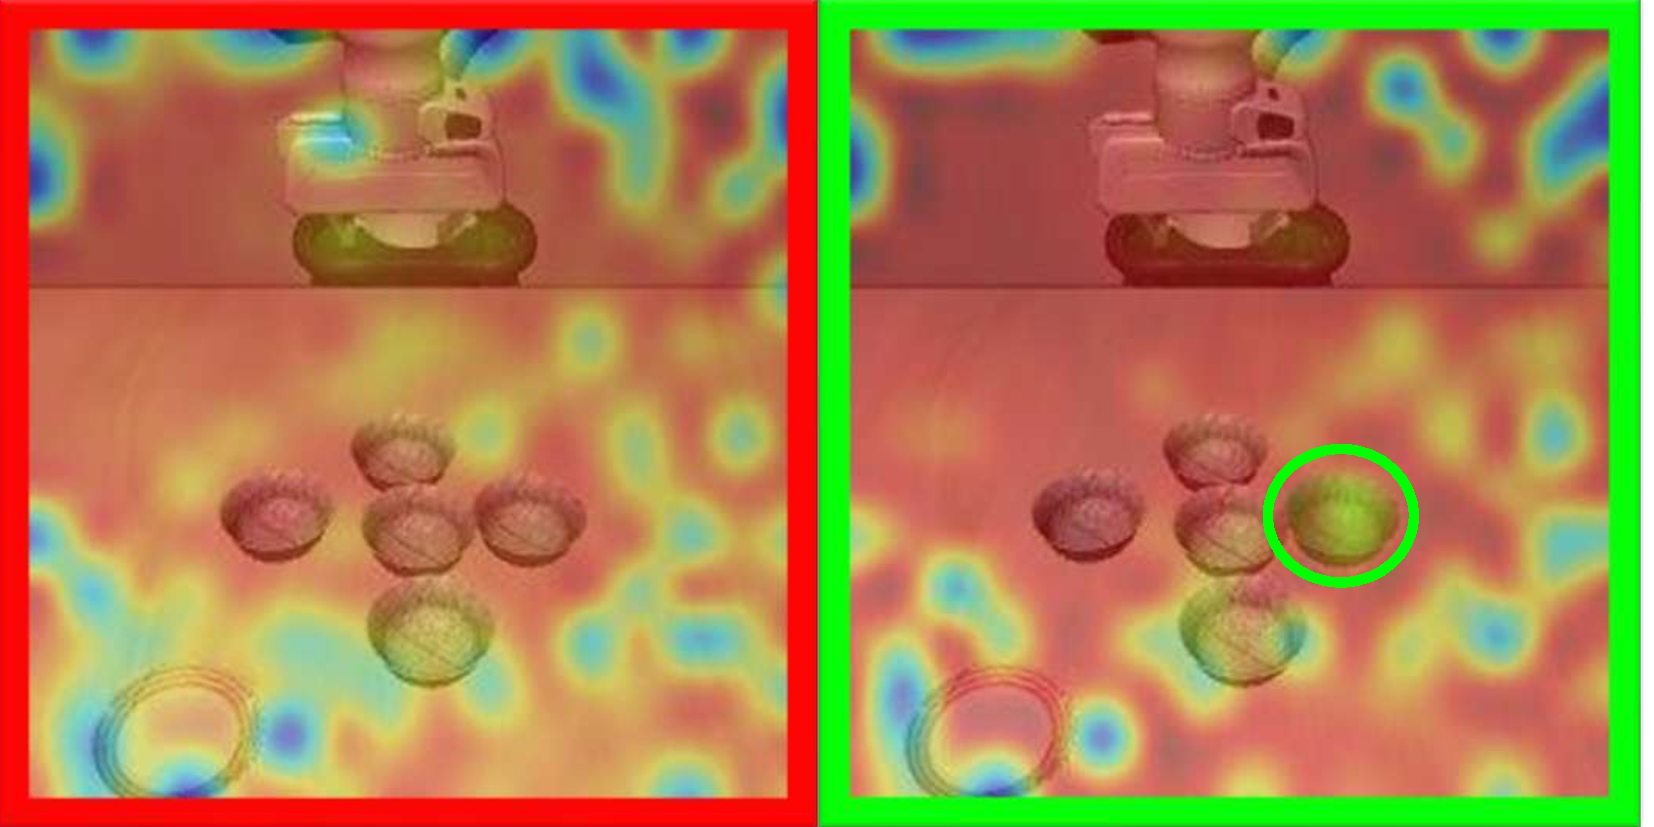
\includegraphics[width=\textwidth]{figure/visual_overlay.pdf}
         \caption{视觉叠加}
         \label{fig:sub1}
     \end{subfigure}
     \hfill
     \begin{subfigure}[b]{0.15\textwidth}
         \centering
         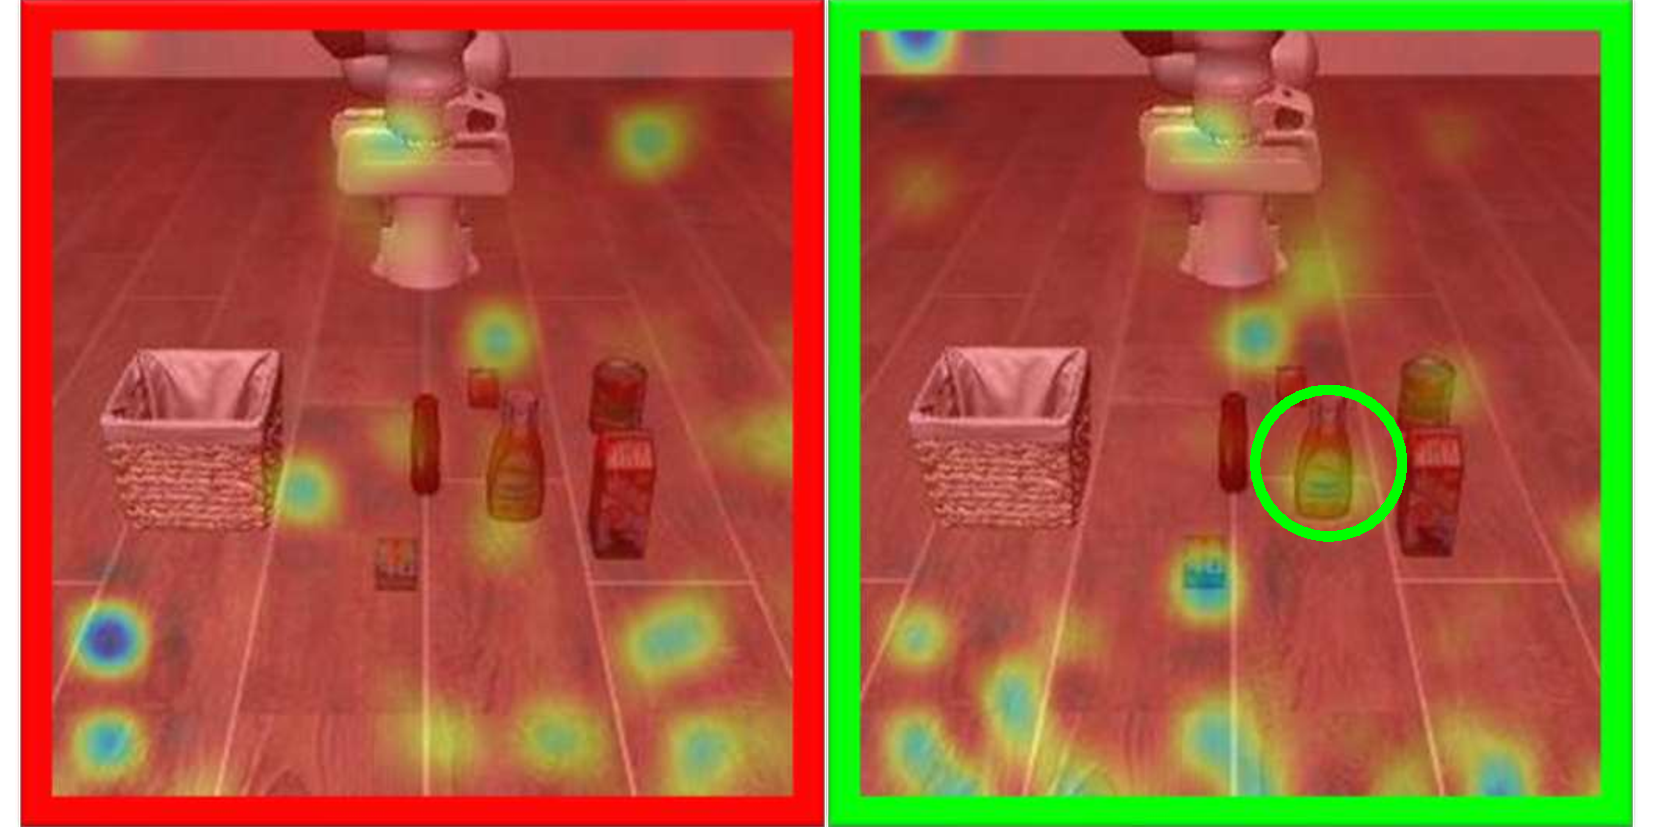
\includegraphics[width=\textwidth]{figure/prompt_simplify.pdf}
         \caption{提示简化}
         \label{fig:sub2}
     \end{subfigure}
     \hfill
     \begin{subfigure}[b]{0.15\textwidth}
         \centering
         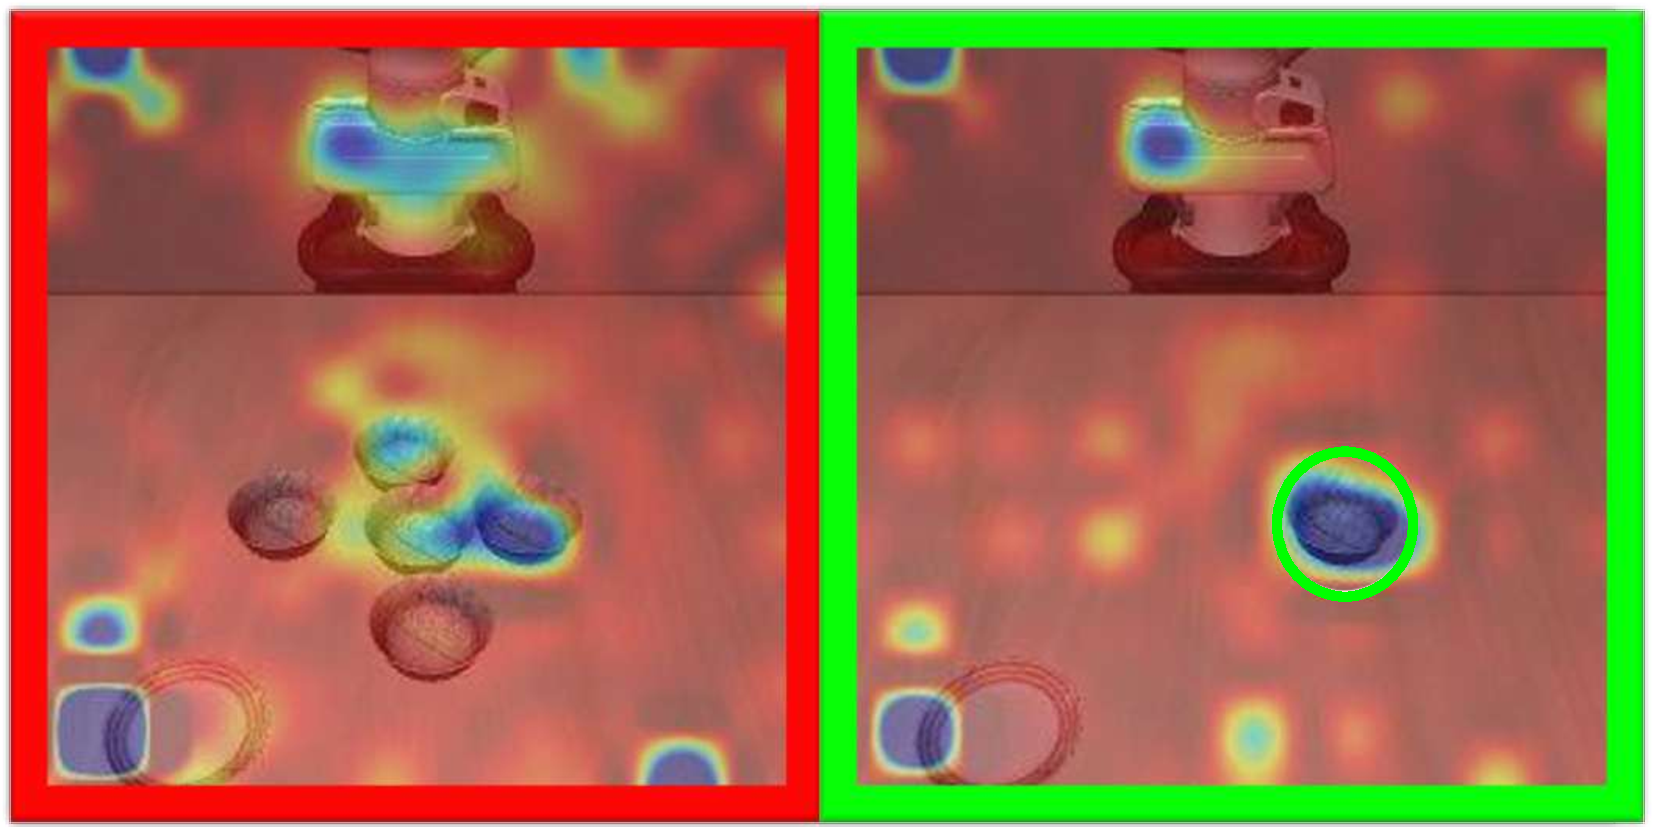
\includegraphics[width=\textwidth]{figure/distractor_attention.pdf}
         \caption{干扰物移除}
         \label{fig:sub3}
     \end{subfigure}
     \hfill
     \begin{subfigure}[b]{0.45\textwidth}
         \centering
         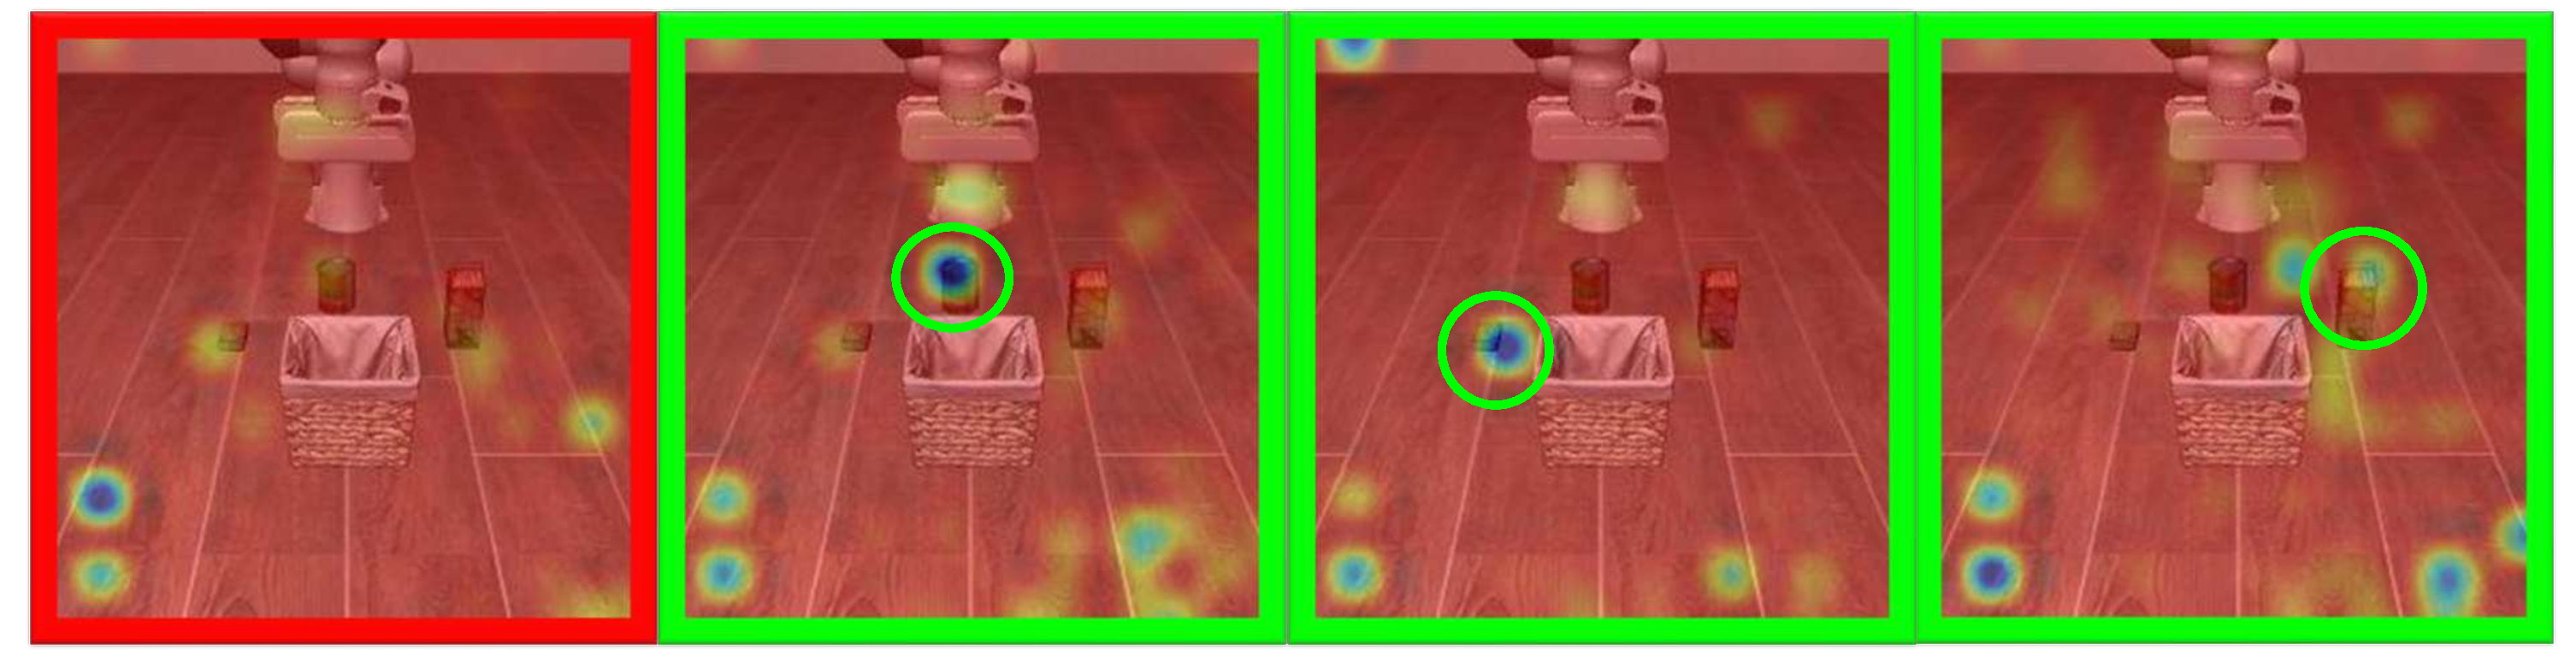
\includegraphics[width=\textwidth]{figure/long_task.pdf}
         \caption{长时程任务}
         \label{fig:sub4}
     \end{subfigure}

    \caption{\textbf{不同输入下的注意力图。}红色/蓝色表示高/低注意力；绿色圆圈标示干预位置，而不是热力图数值。
    基线（红框）的关注较为分散，而 MCP 干预（绿框）通过视觉提示、提示简化、杂物过滤和子任务分解，改善了物体定位与边界勾勒。}
     \label{fig:attention_maps}
     \vspace{-1.5em}
\end{figure}

为克服这些局限，我们将\textbf{\sys}定义为面向冻结 VLA 模型的记忆增强策略外壳。
它不更新参数，而是在基础策略外包裹检索落地的诊断、工具介导的感知--语言干预和控制流恢复，从而在查询时调节观测、指令与执行上下文。
\sys\ 通过解耦架构实现上述要求：三个在线组件负责任务干预，一个异步离线双阶段记忆巩固模块负责长期能力改进。

\emph{(i)} \textbf{长期经验对齐：}
如图~\ref{fig:attention_maps} 所示，OOD 失败往往源于感知“注意力漂移”，而非运动能力的极限：环境或语言噪声会扰乱冻结 VLA 的关注点。
为此，\sys\ 维护一个包含成功与失败执行的\textbf{长期记忆库}，并回忆曾解决类似失败的输入级调整。
通过 MCP 工具干预~\cite{MCP}，\sys\ 无需更新参数即可使当前感知与以往经验对齐。

\emph{(ii)} \textbf{因果失败归因：}
对于仅靠检索无法解决的失败，\sys\ 在成功和失败经历上执行\textbf{对比式双记忆检索}。
视觉--语言编排器比较两者，以识别感知歧义或规划偏差，并指导有针对性的干预。

\emph{(iii)} \textbf{动态工具编排：}
MCP 将诊断结果转换为\textbf{动态编排}的模块化工具链。
编排器根据因果诊断组合 MCP 序列，以修正视觉输入或改进任务上下文。

\emph{(iv)} \textbf{记忆巩固：}
每项任务结束后，一个离线工作流在不中断执行的情况下更新记忆。
\textbf{初始诊断}对最新轨迹进行归因，并将其写入双记忆库；\textbf{记忆巩固}检索相似历史，通过跨任务差分分析改进已有归因和干预方案。
这一自纠正闭环可防止知识停滞，并改善后续干预。

在标准 \textbf{LIBERO-PRO}~\cite{liberopro} 基准和我们定制的 \textbf{LIBERO-\sys} 套件上进行的实证评估表明，本框架无需微调即可持续增强多种 VLA 模型的上下文内自适应能力。
在基础模型经常因感知与语言噪声失败的 LIBERO-\sys\ 上，\sys\ 使性能平均提升 $\mathbf{59.3\%}$，其中长时程任务的绝对提升最高达到 $89.1\%$。
类似地，在 LIBERO-PRO~\cite{liberopro} 上，\sys\ 有效弥合了由布局和语义偏移造成的分布差距（基线成功率约为 $0\%$），加权平均提升 $\mathbf{54.5\%}$。
这些结果表明，\sys\ 是一种可即插即用、能够稳健应对 OOD 机器人挑战的方案。

总之，本文有三项贡献：
\begin{enumerate}
    \item \textbf{归因驱动的记忆与可扩展干预架构：}
    我们提出一个克服传统 RAG“成功偏置”的闭环架构。\sys\ 使用对比式双记忆检索诊断失败，并以动态编排的 MCP 工具执行针对性干预，从而形成一个无参数更新、可即插即用的 VLA 模型鲁棒化框架。

    \item \textbf{异步系统设计：}
    我们将任务级干预与长期知识改进解耦：在线流水线执行归因引导的 MCP 干预，离线巩固则更新归因和记忆，在不中断推理或更新参数的情况下提炼可靠先验。

    \item \textbf{上下文内自适应与实验结果：}
    在多种任务与骨干模型上，\sys\ 将推理从冻结策略转移到持续演化的记忆库和可扩展工具，从而改善性能与上下文内自适应，并在传统 VLA 策略通常失败的 OOD 条件下保持鲁棒性。
\end{enumerate}

\endinput

\vspace{-1em}
\section{相关工作}
\label{sec:related_work}

\subsection{VLA 模型与泛化挑战}

近年来，机器人学习发生了范式转变：从专门的策略网络走向通用 VLA 模型。
$\pi_0$~\cite{pi0} 和 OpenVLA~\cite{openvla} 等先驱工作利用海量网络规模数据集（例如 Open-X Embodiment~\cite{openx}）实现端到端机器人控制，将视觉编码器（例如 SigLIP~\cite{siglip}）与大语言模型相结合，把开放词汇指令转换为精确的连续动作。
然而，通过微调（例如 X-VLA~\cite{xvla}）使这些模型适应 OOD 场景会产生高昂的计算成本，因此需要无需更新权重、参数高效且可即插即用的泛化方法。

\subsection{机器人领域的 RAG 与上下文学习}

为在不微调的情况下提高适应能力，研究者已将 RAG 和上下文学习（ICL）引入机器人领域。
RICL~\cite{ricl} 和 MemER~\cite{memer} 等框架通过向量数据库检索相关历史示范，并把它们作为上下文提示附加到策略执行中，从而通过最近邻模仿适应新任务。
这些方法虽然能有效利用外部记忆，却只关注成功轨迹，忽略了失败经历的诊断价值。这说明我们需要一种同时利用成功与失败进行对比式指导的双记忆结构。

\subsection{上下文内自适应智能体框架}

除被动检索轨迹外，近期研究还探索了让 LLM 和 VLM 作为具有外部工具访问能力的高层规划器。
Code-as-Policies~\cite{cap} 为层级任务生成可执行 Python 代码，VoxPoser~\cite{voxposer} 将指令落地为用于运动规划的三维空间价值图，而 MOKA~\cite{moka} 则通过视觉提示在图像上标注可供性。
这些框架虽然能把复杂指令分解为可在上下文中自适应的可执行原语，但缺少闭环适应所需的经验记忆与动态纠错能力。

\endinput

\section{方法}

\begin{figure*}[t]
  \centering
  \vspace{0.5em}
  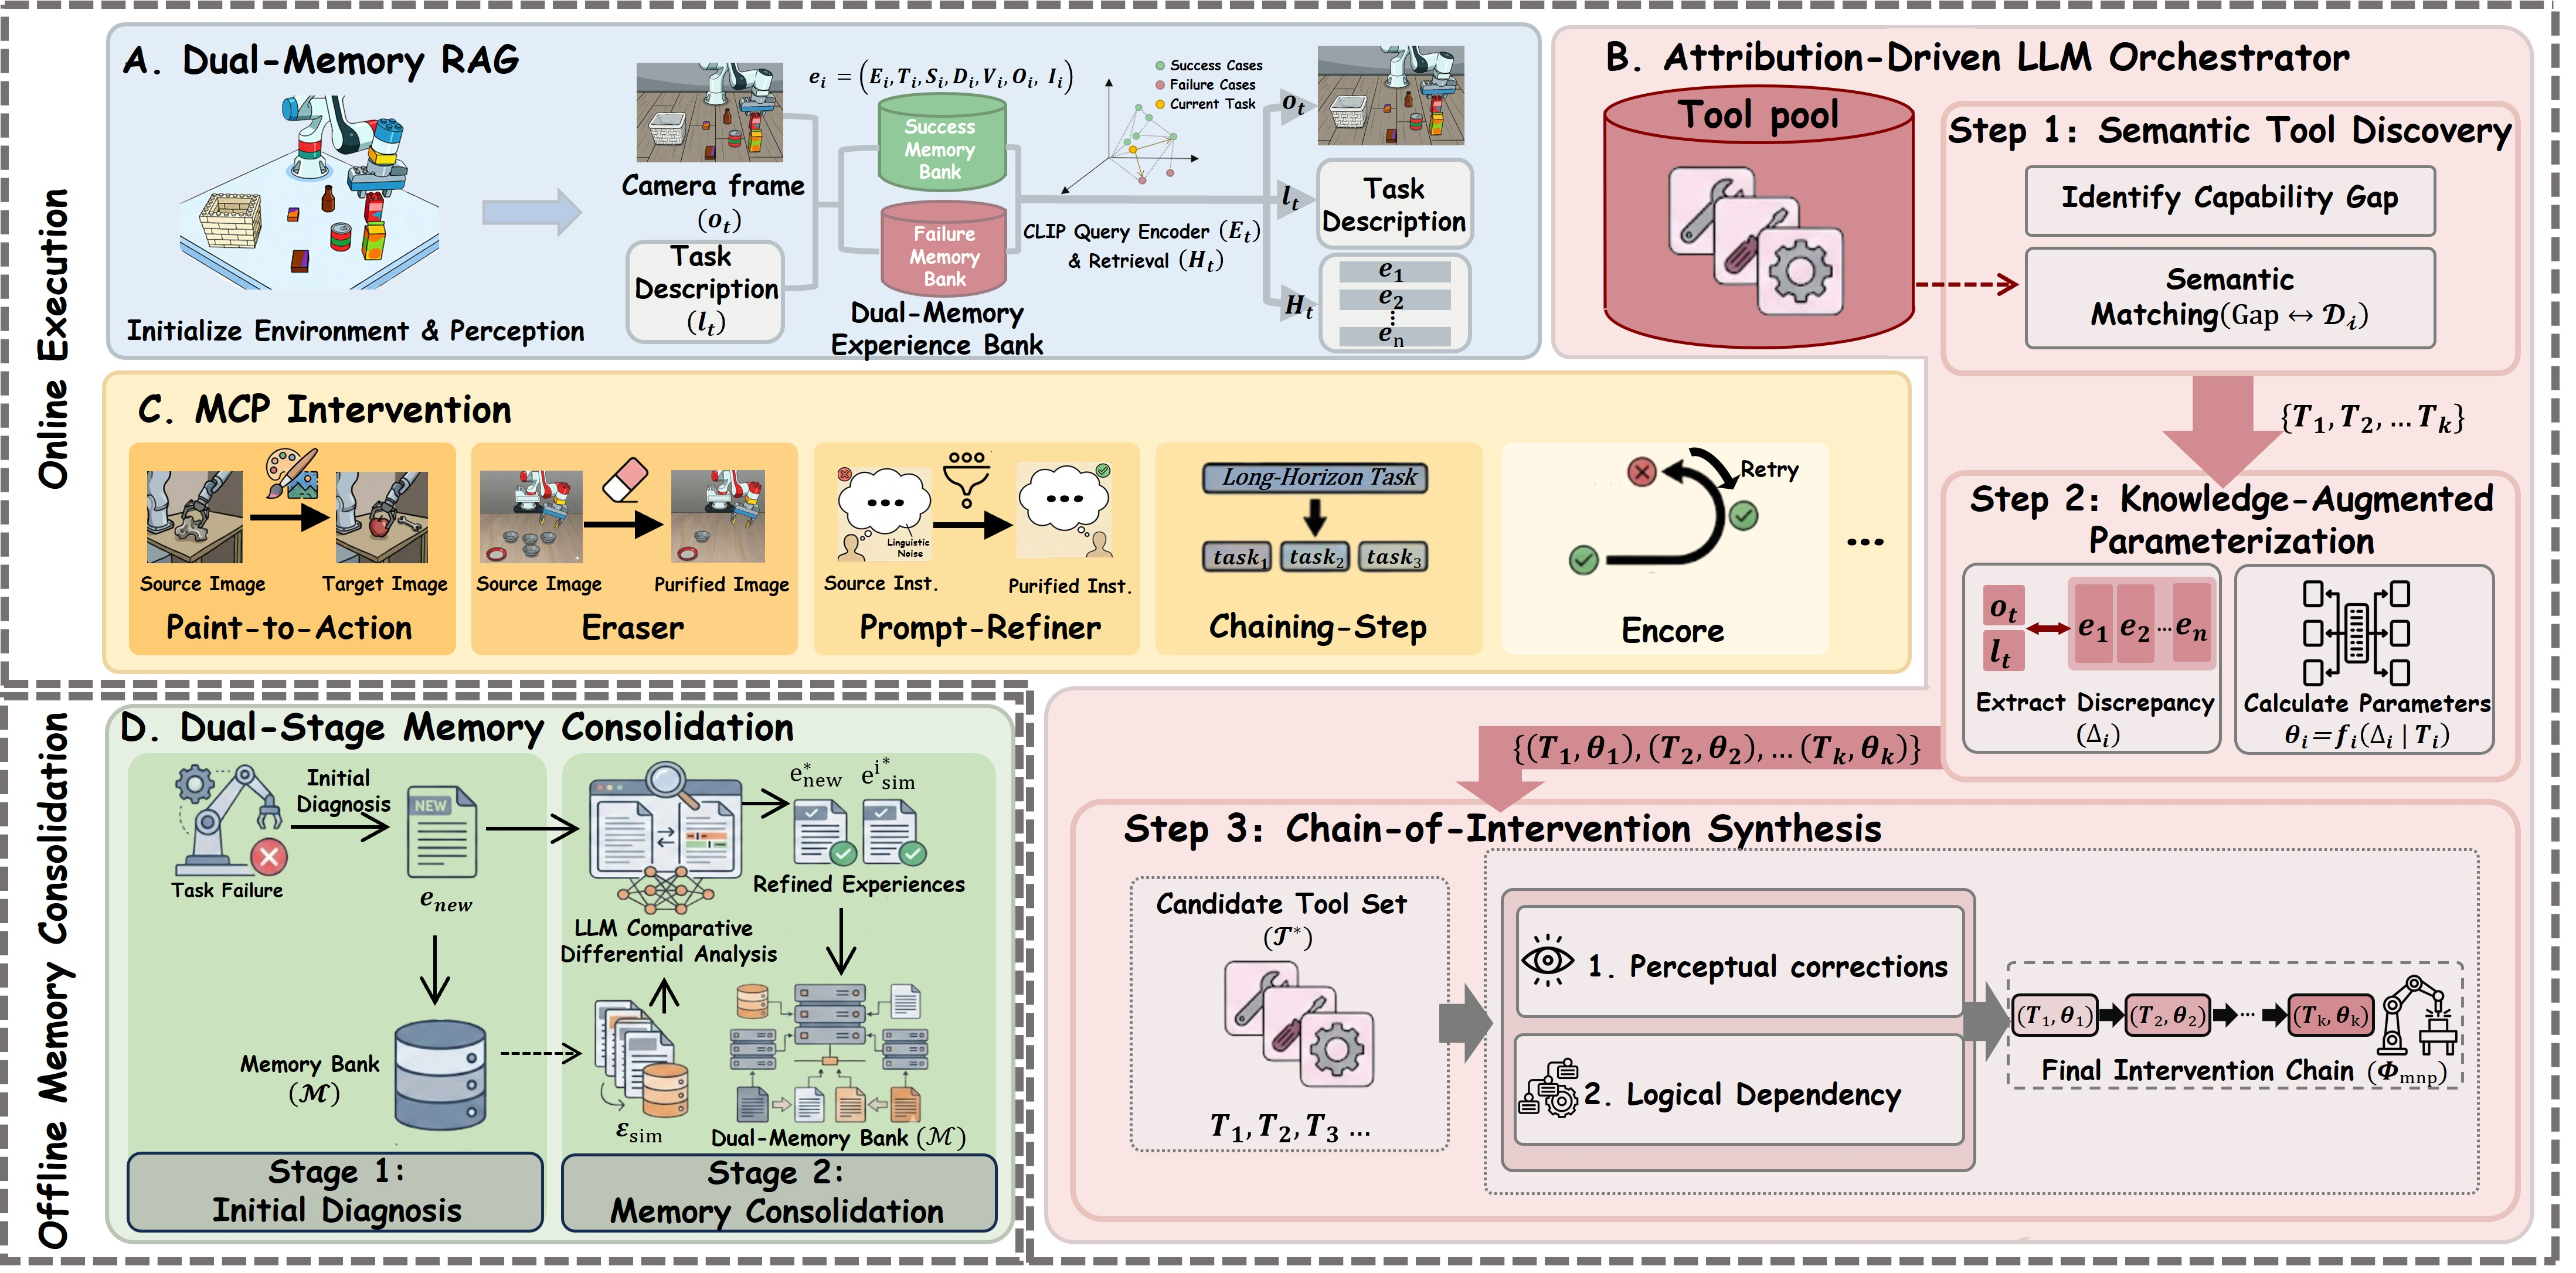
\includegraphics[width=0.85\linewidth]{figure/framework.jpg}
  \caption{\textbf{\sys\ 框架。}给定观测和指令，双记忆 RAG 从双记忆库检索相关经验。视觉--语言编排器选择 MCP 工具、估计参数 $\theta$，并合成由可扩展 MCP 工具执行的干预链。执行后，异步记忆巩固更新记忆库，闭合迭代改进回路。}
  \vspace{-1.5em}
  \label{framework}
\end{figure*}

本节介绍\textbf{\sys}框架。如图~\ref{framework} 所示，它由\textbf{在线执行工作流}和\textbf{离线记忆巩固工作流}组成。

\paragraph{在线执行工作流}
在线工作流通过三个模块实现鲁棒的任务级自适应：
\textbf{(1) 双记忆 RAG} 从双记忆库检索成功指导和失败警示；
\textbf{(2) 归因驱动的视觉--语言编排器}诊断障碍，并选择由归因指导的干预；
\textbf{(3) MCP 干预}通过调节感知和语言输入的可扩展工具执行这些干预。

\paragraph{离线记忆巩固工作流}
作为在线执行的补充，离线工作流进行\textbf{双阶段记忆巩固}。
它将新观测到的成功和失败轨迹提炼为结构化记忆并更新双记忆库，从而无需更新参数即可持续改进。

这两个工作流共同构成一个闭环自适应系统。
\vspace{-0.5em}
\[
\underbrace{
    \overbrace{\text{Obs.} \rightarrow \text{Retr.} \rightarrow \text{Dec.} \rightarrow \text{Orch.}}^{\substack{\text{任务级} \\ (\text{每项任务一次})}} \rightarrow \overset{\substack{\text{片段级} \\ (\text{每 } N \text{ 步})}}{\text{Exec.}}
}_{\text{在线}}
\rightarrow
\underbrace{\text{Consol.}}_{\text{离线}}
\]
下面详细介绍各模块。

\subsection{双记忆 RAG}
\label{dual memory}

图~\ref{framework}A 展示了一个检索增强的双记忆库，它使用先前的成功和失败经验为编排器的推理提供落地依据。
其\textbf{双重}设计将成功/失败经验分开以进行对比式归因，并通过双阶段巩固改进每个条目（第~\ref{Evolution} 节）。

下面介绍记忆库的构建过程及其检索机制。

\subsubsection{双记忆存储设计}

我们构建一个双分区记忆库：
\begin{equation}
\mathcal{M} = \mathcal{M}_{succ} \cup \mathcal{M}_{fail},
\end{equation}
其中，$\mathcal{M}_{succ}$ 将成功干预存为正向指导，$\mathcal{M}_{fail}$ 则将带有归因信号的失败尝试存为负面证据，以支持对可复用策略与应避免模式进行对比推理。

第~\ref{dual memory ablation} 节的消融表明，单分区记忆会导致规划不稳定或低效，而同时使用两个分区能够减少推理轮数及其方差。

每个经验条目 $e_i \in \mathcal{M}$ 都以半结构化模式存储：固定的核心模式辅以可扩展辅助字段：
\vspace{-0.5em}
\begin{equation}
e_i = \big(
\overbrace{E_i, T_i, S_i, D_i, V_i, O_i}^{\text{固定模式}},
\mathcal{I}_i
\big),
\end{equation}
\begin{itemize}
    \item $E_i$：任务实例的多模态嵌入；
    \item $T_i$：自然语言任务描述；
    \item $S_i \in \{0,1\}$：成功指示量；
    \item $D_i$：诊断标注（失败时非空）；
    \item $V_i$：执行视频的关键帧表征；
    \item $O_i$：表示为物体--属性对的结构化场景；
    \item $\mathcal{I}_i$：可扩展的结构化元数据包。
\end{itemize}

元数据包 $\mathcal{I}_i$ 存储 \texttt{key\_frame\_range}、\texttt{success\_max\_step} 和 \texttt{rollback} 等工具执行参数，同时允许随工具或推理信号演化而加入新字段。

\subsubsection{基于相似度的检索策略}

我们使用预训练 CLIP 编码器~\cite{CLIP} $E(\cdot, \cdot)$，将当前任务上下文（初始观测 $o_t$ 与指令 $l_t$）投影到联合嵌入空间。
检索形式化为：
\begin{equation}
\mathcal{H}_t = \text{Top-}k\Big(\text{Sim}\big(E(o_t, l_t), \{E_i \mid e_i \in \mathcal{M}\}\big)\Big),
\end{equation}
$\mathcal{H}_t$ 同时包含成功样例与失败先例，为归因驱动推理提供\textbf{正向指导}和\textbf{负向反事实}。

三元输入 $(\mathcal{H}_t, o_t, l_t)$ 为编排器诊断差异并安排适当干预工具的顺序提供了必要的落地依据。
\vspace{-0.5em}

\subsection{归因驱动的视觉--语言编排器}

如图~\ref{framework}B 所示，归因驱动的视觉--语言编排器是 \sys\ 的决策核心。
它由 Qwen3-VL-32B 驱动；这里把该多模态大语言模型（MLLM）用作视觉--语言模型，对观测、指令和检索到的视觉--语义记忆进行联合推理，以诊断执行失败并编排 MCP 干预。

\subsubsection{语义工具发现与意图对齐}

编排器通过度量当前状态 $o_t$ 与检索原型 $\mathcal{H}_t$ 之间的能力差距来确定干预。
给定语义工具描述 $\{\mathcal{D}_i\}_{i=1}^N$，它执行零样本匹配以选择候选工具集：
\begin{equation}
    \mathcal{T}_{1:k}= \text{Match}\big(\Delta_{g}, \{\mathcal{D}_i\}_{i=1}^N\big), \quad \Delta_{g} = \text{Gap}(o_t, \mathcal{H}_t),
\end{equation}
由此选择功能与诊断出的失败原因一致的工具。

\subsubsection{知识增强的参数化}
\label{Knowledge-Augmented Parameterization}

选定工具后，编排器从多模态上下文差异 $\Delta$ 推导执行参数 $\theta_i$：
\begin{equation}
 \theta_i = f(\Delta_i \mid T_i), \quad \Delta_i = \text{Gap}(o_t, l_t, \mathcal{H}_t\mid T_i),
\end{equation}
其中 $f$ 表示面向特定工具取值的映射函数。
具体而言，$\Delta$ 描述当前观测 $o_t$ 和指令 $l_t$ 相对于历史先验 $\mathcal{H}_t$ 在视觉、语义和时间维度上的偏差。
表~\ref{tab:parameterization_formal} 总结了如何把这些定量差异映射为各工具的具体执行参数 $\theta_i$。

\begin{table}[htbp]
\vspace{-1.5em}
\centering
\caption{面向特定工具的参数化映射。}
\label{tab:parameterization_formal}
\footnotesize
\renewcommand{\arraystretch}{1.25}
\begin{tabularx}{\columnwidth}{@{} l X l @{}}
\toprule
\textbf{工具} & \textbf{相对于 $\mathcal{H}_t$ 的差异 $\Delta$} & \textbf{$\theta_i$} \\
\midrule
Paint  & 与历史均值的特征距离。         & $C,\,M,\,A_{mask}$ \\
Eraser & 相对背景模型的新颖几何结构。   & $D,\,D_{masks}$ \\
Prompt & 与成功模式不匹配的指令。       & $\mathcal{S}_{origin}$ \\
Chain  & 子事件级对齐。                 & $(N_{e},N_{b})_k$ \\
Encore & 与历史失败轨迹的相似度。       & $[s_s,s_e],\,N_w$ \\
\bottomrule
\end{tabularx}
\vspace{3pt}
\begin{flushleft}
\scriptsize
\textbf{$C$}：颜色/纹理；\enspace
\textbf{$M$}：材质；\enspace
\textbf{$A_{mask}$}：目标物体掩码；\enspace
\textbf{$D$}：干扰物描述；\enspace
\textbf{$D_{masks}$}：干扰物掩码；\enspace
\textbf{$\mathcal{S}_{origin}$}：原始任务的简化目标；\enspace
\textbf{$N_{e,b}$}：执行/缓冲步数；\enspace
\textbf{$s_{s,e}$}：开始/结束步；\enspace
\textbf{$N_w$}：等待时长。
\end{flushleft}
\vspace{-0.5em}
\end{table}

最终输出是一组参数化干预：
\begin{equation}
\mathcal{T}^* = \{(T_1, \theta_1), (T_2, \theta_2), \dots, (T_k, \theta_k)\}.
\end{equation}

\subsubsection{干预链合成}

随后，编排器将这些工具合成为一个有序干预链：
\begin{equation}
\begin{aligned}
\Phi_{\text{mcp}} &= \text{Orchestrate}(\mathcal{T}^*) \\
&= \big\langle (T_1, \theta_1) \rightarrow (T_2, \theta_2) \rightarrow \dots \rightarrow (T_k, \theta_k) \big\rangle.
\end{aligned}
\end{equation}

编排遵循两个原则：
\begin{enumerate}
    \item \textbf{感知优先：}感知修正（例如 \textit{Paint-to-Action}、\textit{Eraser}）先于物理恢复（例如 \textit{Encore}），以避免因错误感知而反复失败。
    \item \textbf{逻辑依赖：}先移除因果干扰，再进行下游推理和执行。
\end{enumerate}

\noindent\textbf{例如}，当视觉偏移与执行停滞同时发生时，编排器生成
\textbf{$\text{Paint-to-Action} \rightarrow \text{Encore}$}，
使感知修正先于回滚。

\subsection{MCP 干预}

如图~\ref{framework}C 所示，该模块通过感知或物理动作执行干预链 $\Phi_{\text{mcp}}$。
我们针对常见 VLA 失败（例如分布偏移和因果干扰）实例化五种 MCP 工具，同时为新的失败类型保留可即插即用的扩展能力。

\subsubsection{Paint-to-Action：视觉域偏移}
\begin{figure}[htbp]
    \centering
    \vspace{-0.5em}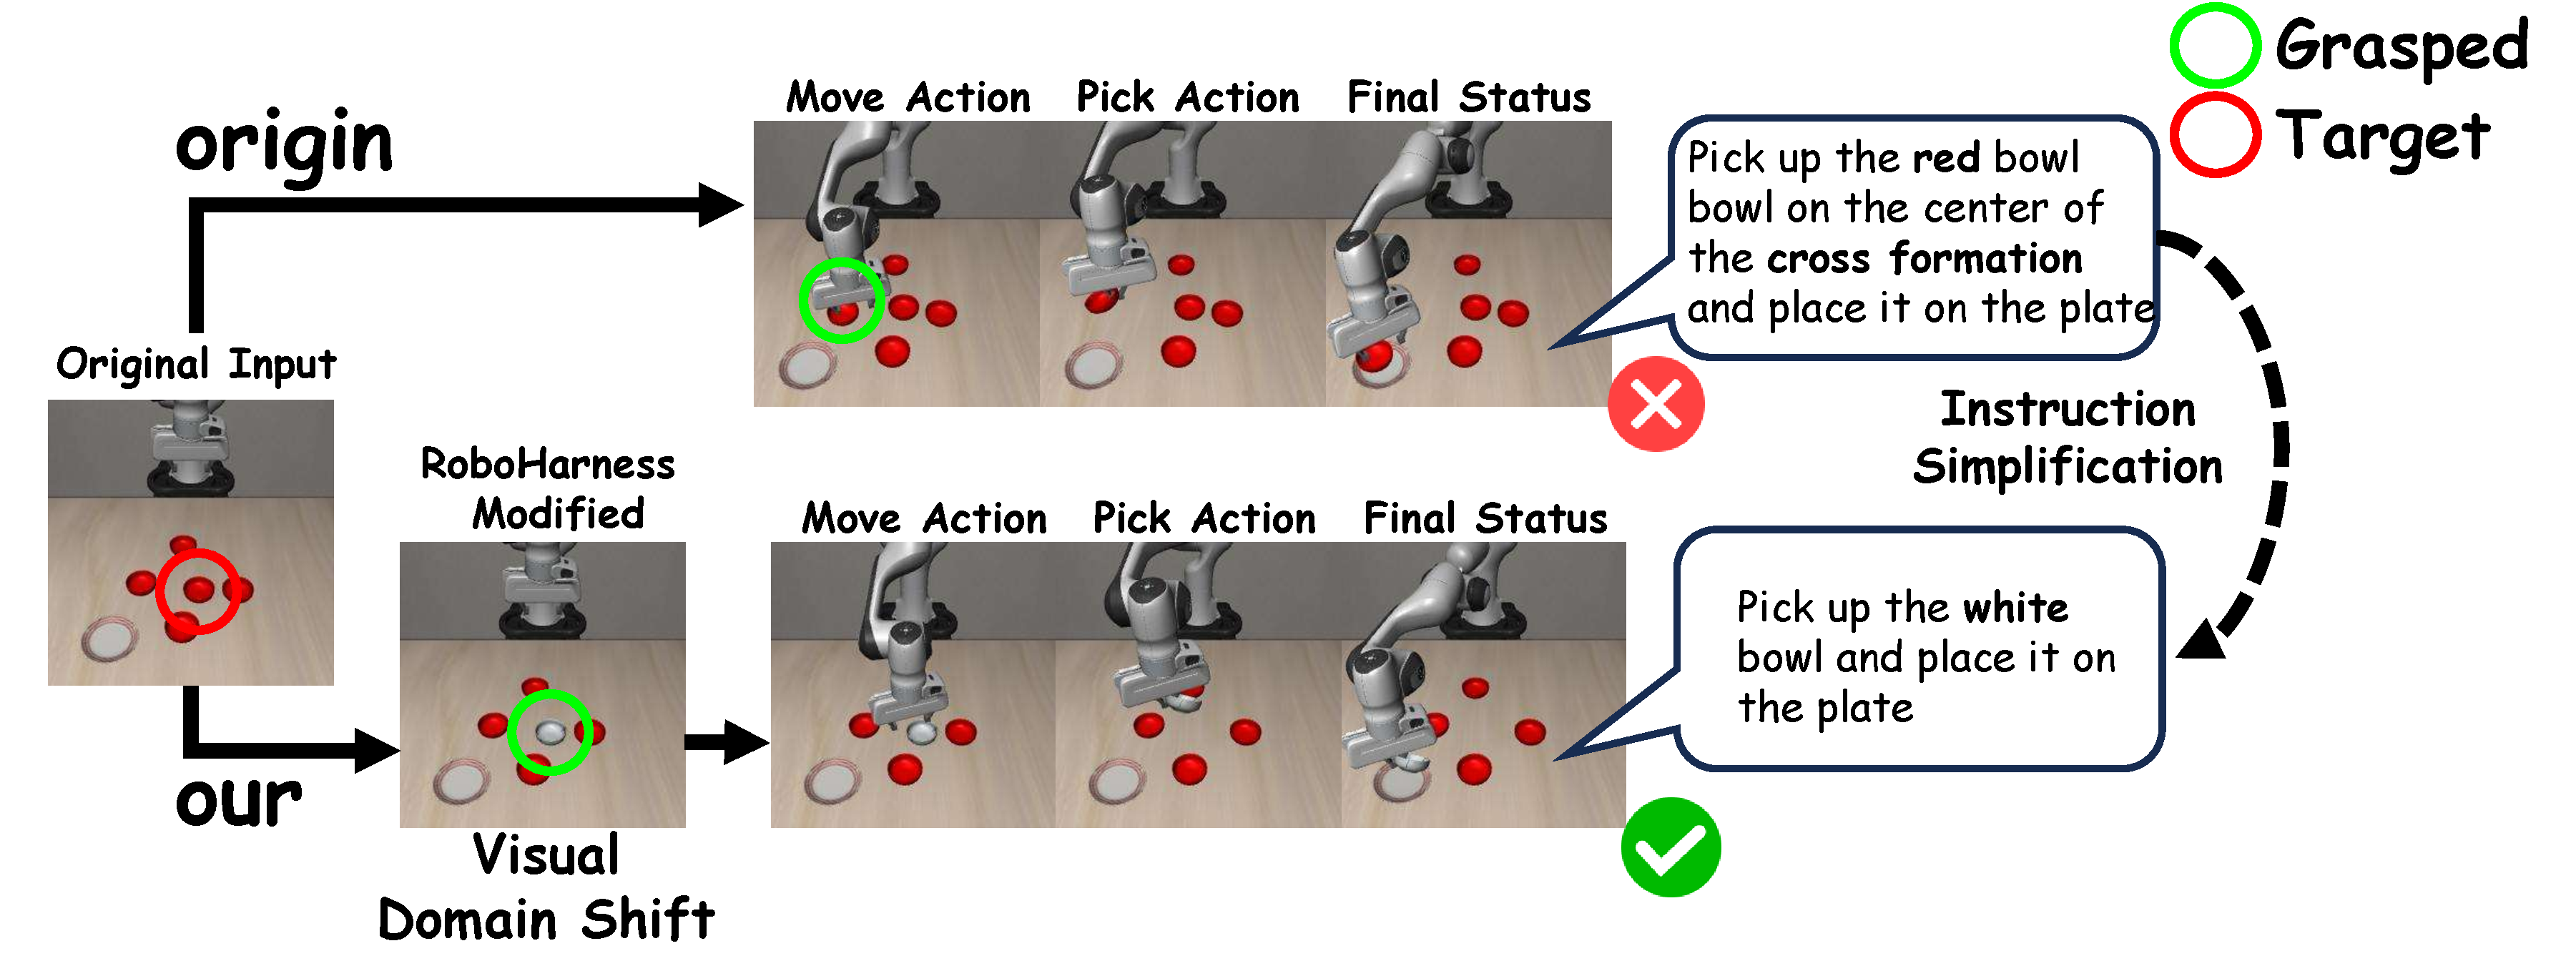
\includegraphics[width=0.95\columnwidth]{figure/visual_shift.pdf}
    \caption{\textbf{视觉聚焦。}处理复杂操作环境中的视觉偏移。}
    \label{fig:visual_shift}
    \vspace{-1em}
\end{figure}
Paint-to-Action 执行非参数域自适应：
\begin{equation}
o_t' = \text{Paint-to-Action}(o_t, \theta_{\text{dist}}).
\end{equation}
它通过 \texttt{visual\_overlay} 和 \texttt{replace\_texture} 实现。
编排器推导 $\theta_{\text{dist}}$，SAM3~\cite{sam3} 分割目标区域，再通过高对比度掩码或成功轨迹中的纹理（\texttt{rag\_success}）缓解偏移（图~\ref{fig:visual_shift}）。

\subsubsection{Eraser：因果混淆}
\begin{figure}[htbp]
    \centering
    \vspace{-0.5em}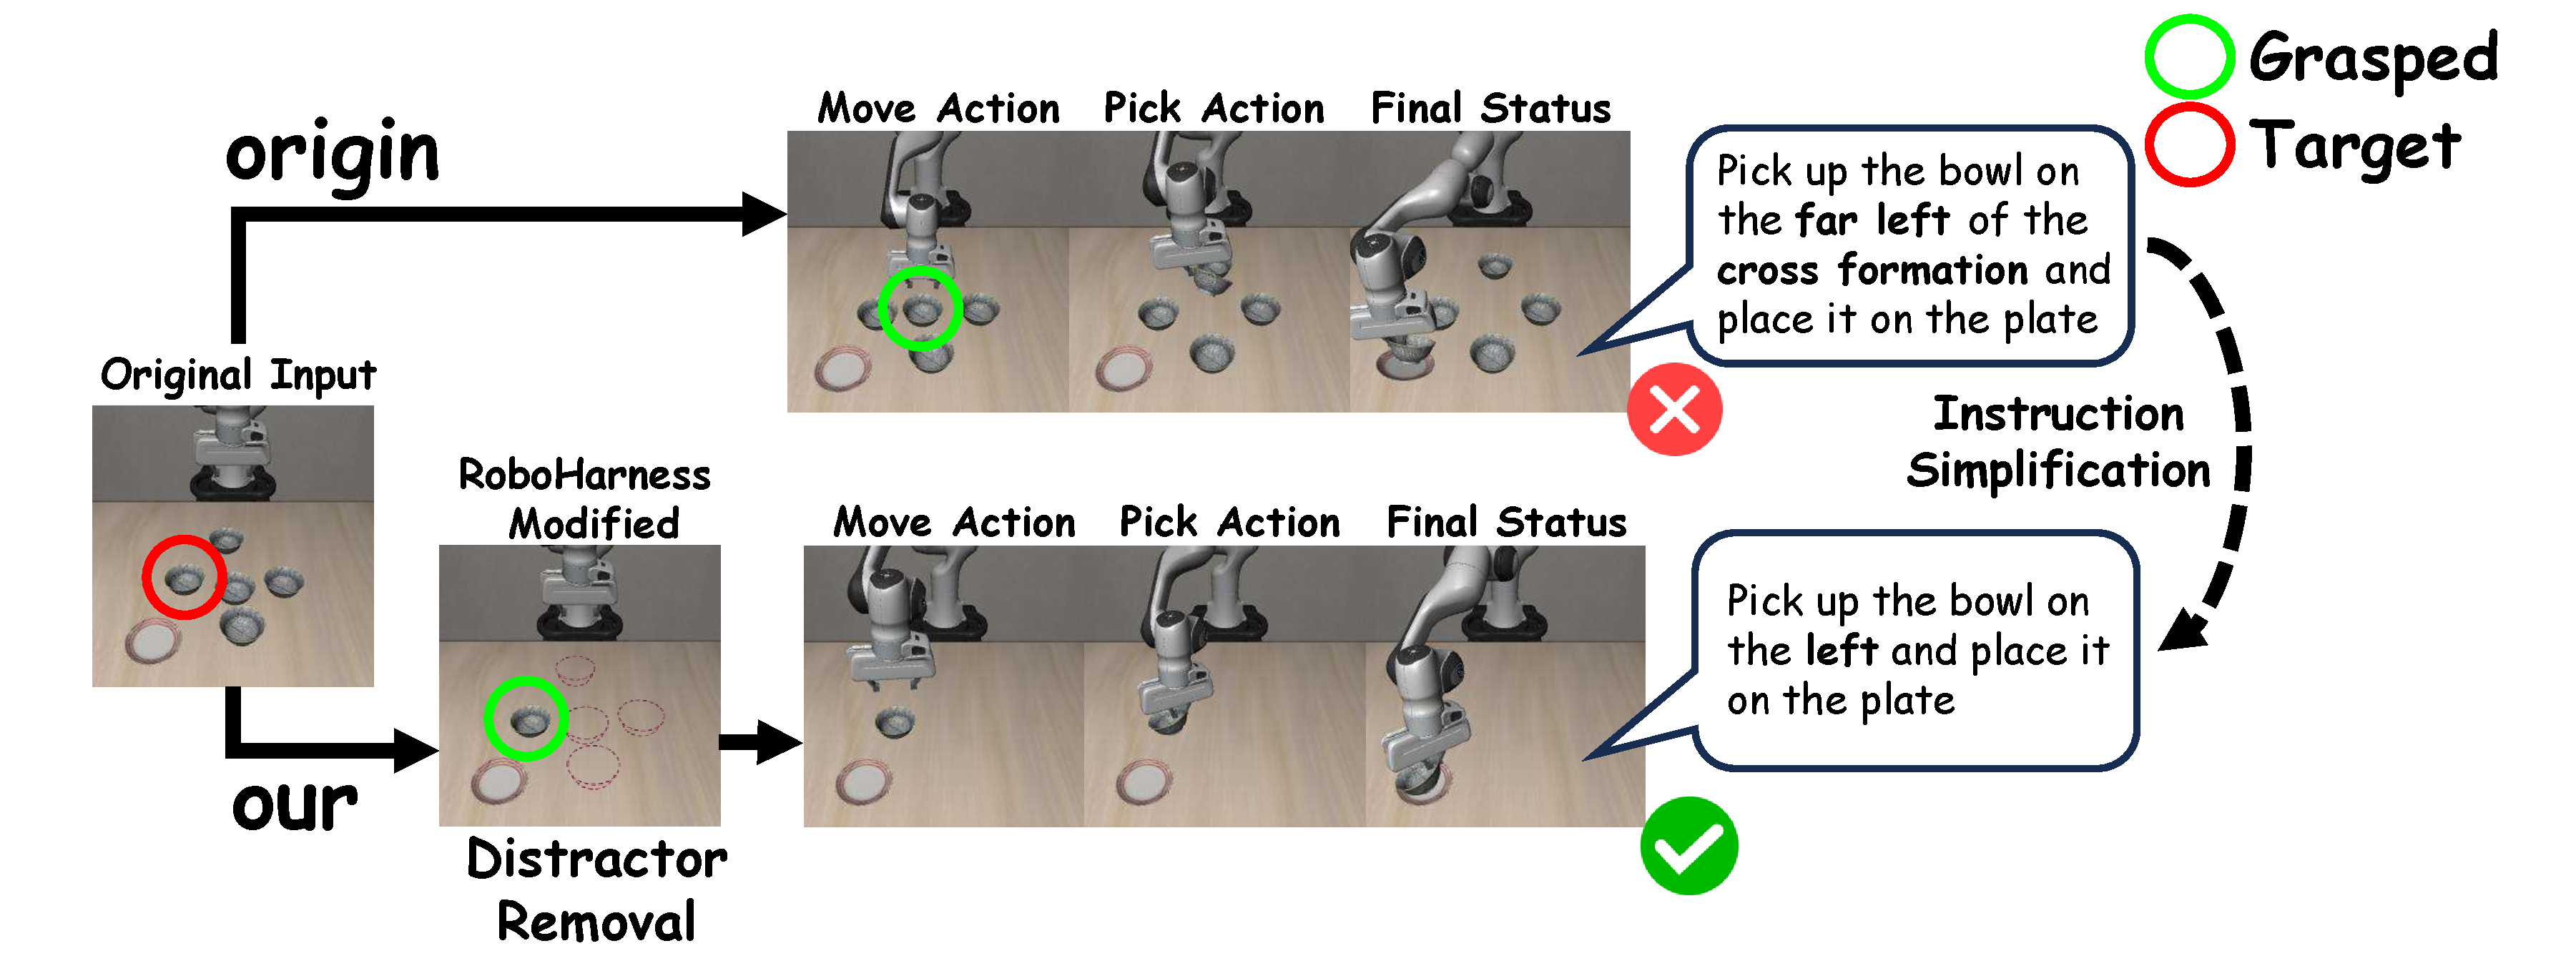
\includegraphics[width=0.95\columnwidth]{figure/remove_distract.pdf}
    \caption{\textbf{杂物移除。}擦除无关干扰物以缓解因果混淆。}
    \label{fig:remove_distract}
    \vspace{-1em}
\end{figure}
Eraser 通过 $\theta_{\text{conf}}$ 移除无关物体：
\begin{equation}
o_t' = \text{Eraser}(o_t, \theta_{\text{conf}}).
\end{equation}
使用 \texttt{remove\_distractor} 时，编排器根据 $o_t$ 和 $\mathcal{H}_t$ 识别干扰物，SAM3~\cite{sam3} 提取掩码，OpenCV Telea 修复算法则在策略推理前移除这些干扰物（图~\ref{fig:remove_distract}）。

\subsubsection{Prompt-Refiner：指令模式不匹配}
\begin{figure}[htbp]
    \centering
    \vspace{-0.5em}
    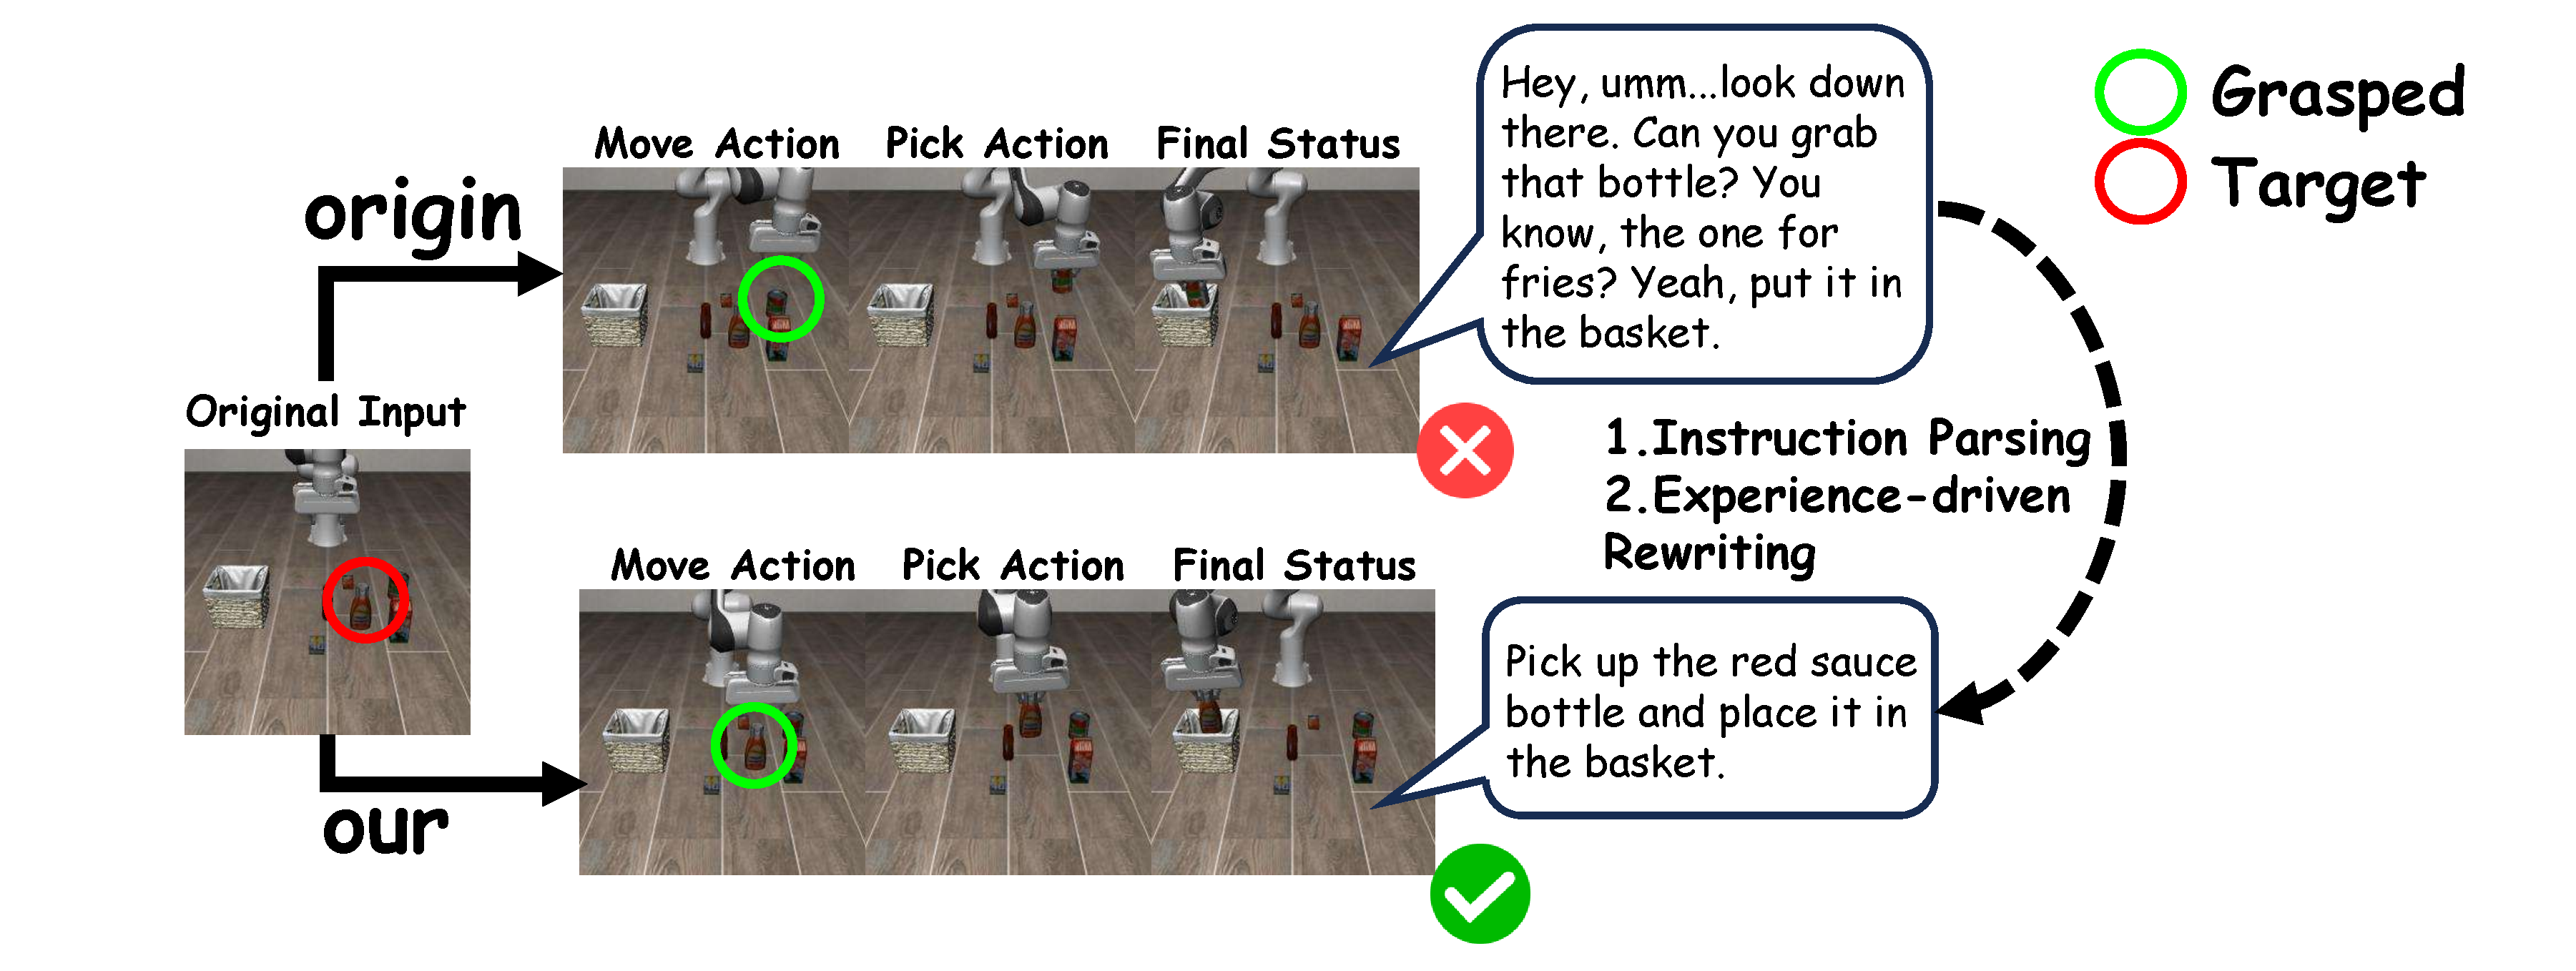
\includegraphics[width=0.95\columnwidth]{figure/prompt_understanding.pdf}
    \caption{\textbf{噪声提示。}将偏离历史成功经验模式的指令改写为简洁、可执行的命令。}
    \label{fig:prompt_understanding}
    \vspace{-1em}
\end{figure}
Prompt-Refiner 改进措辞或任务结构偏离检索成功经验的指令：
\begin{equation}
l_t' = \text{Prompt-Refiner}(l_t, \theta_{\text{lang}}).
\end{equation}
当 $l_t$ 的措辞或任务结构偏离 $\mathcal{H}_t$ 中检索到的成功经验模式时，编排器对其进行改写，生成简洁的 \texttt{refined\_task} 供执行（例如，图~\ref{fig:prompt_understanding} 中的口语化或对话式指令被改写为“Pick\ldots and place\ldots”形式）。

\subsubsection{Chaining-Step：时间复合误差}

Chaining-Step 缩短任务时程：
\begin{equation}
A_{seq}' = \text{Chaining-Step}(A_{seq}, \theta_{\text{chain}}).
\end{equation}
编排器使用 $\mathcal{H}_t$ 将宏观序列 $A_{seq}$ 分解为对齐的子任务，并根据 $\theta_{\text{chain}}$ 指定时间边界（尤其是 $N_e,N_b$）。
以 $A_{seq}'$ 替换 $A_{seq}$ 可缩短执行片段，缓解长时程上下文退化（例如，图~\ref{fig:long_horizon} 中的长任务被拆为更短的子任务，并在其间执行“Reset \& Buffer”）。

\subsubsection{Encore：执行停滞}
\begin{figure}[htbp]
    \vspace{0.5em}
    \centering
    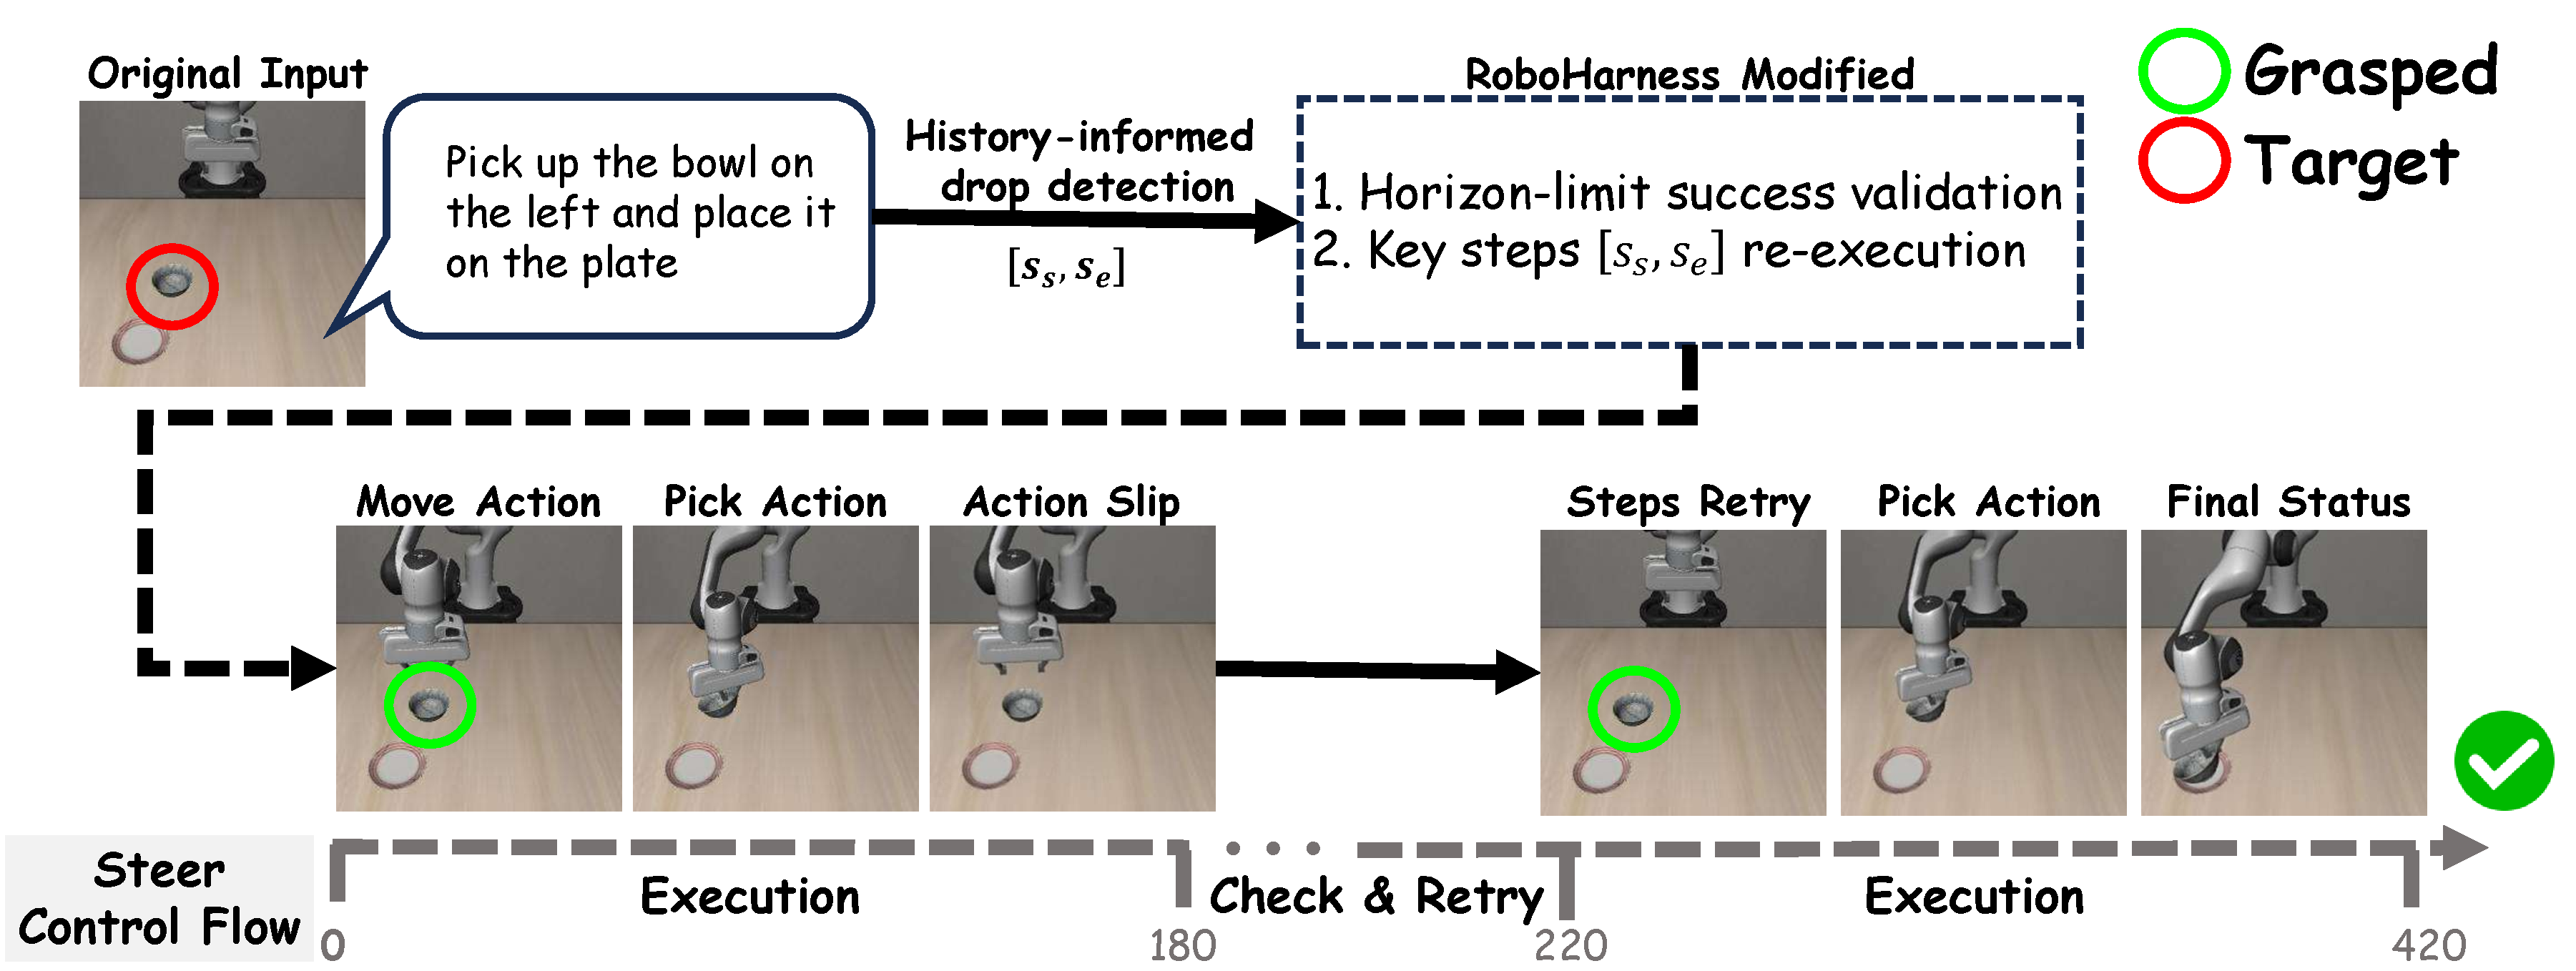
\includegraphics[width=0.95\columnwidth]{figure/encore.pdf}
    \caption{\textbf{Encore。}通过重新执行关键步骤进行恢复。}
    \label{fig:encore}
    \vspace{-1.5em}
\end{figure}
Encore 通过关键状态恢复来解除死锁：
\begin{equation}
s'_t = \text{Encore}(s_t, \theta_{\text{stuc}}).
\end{equation}
其中，$\theta_{\text{stuc}}$（来自 $\mathcal{H}_t$ 中的失败先例）指定重试边界 $[s_s,s_e]$ 和等待时间 $N_w$。
\texttt{encore} 工具重置计数器，并沿平均反向轨迹回滚；若时程上限验证失败，它会从关键帧 $s_s$ 触发“Reset \& Retry”（图~\ref{fig:encore}）。

\subsection{双阶段记忆巩固}
\label{Evolution}

该模块如图~\ref{framework}D 所示，使用双阶段归因机制将最新执行轨迹巩固到双记忆库 $\mathcal{M}$ 中。

\subsubsection{阶段一：初始诊断}

任务终止后，编排器执行初始诊断：
\begin{equation}
e_{new} = \text{InitDiag}(o_t, T_{raw}),
\end{equation}
并存储新经验：
\begin{equation}
\mathcal{M} = \mathcal{M} \cup \{e_{new}\}.
\end{equation}

\subsubsection{阶段二：记忆巩固}

记忆巩固检索最相似的前 $N$ 项经验 $\mathcal{E}_{\text{sim}} = \{e_{\text{sim}}^1, \dots, e_{\text{sim}}^N\}$，以进行跨任务改进：
\begin{equation}
\{e_{\text{new}}^*, e_{\text{sim}}^{1*}, \dots, e_{\text{sim}}^{N*}\} = \text{MemConsol}(e_{\text{new}}, \mathcal{E}_{\text{sim}}),
\end{equation}
其中每个 $e^*$ 都是更新后的经验元组。
编排器进行批次级差分分析，使用新证据纠正历史失败描述并优化修正方案，使 $\mathcal{M}$ 能够迭代自纠正，而非只是单调扩张。

\endinput

\vspace{-0.5em}
\section{实验}

\begin{figure*}[t]
  \centering
  \vspace{0.5em}
  \begin{minipage}[t]{0.66\textwidth}
    \vspace{0pt}
    \centering
    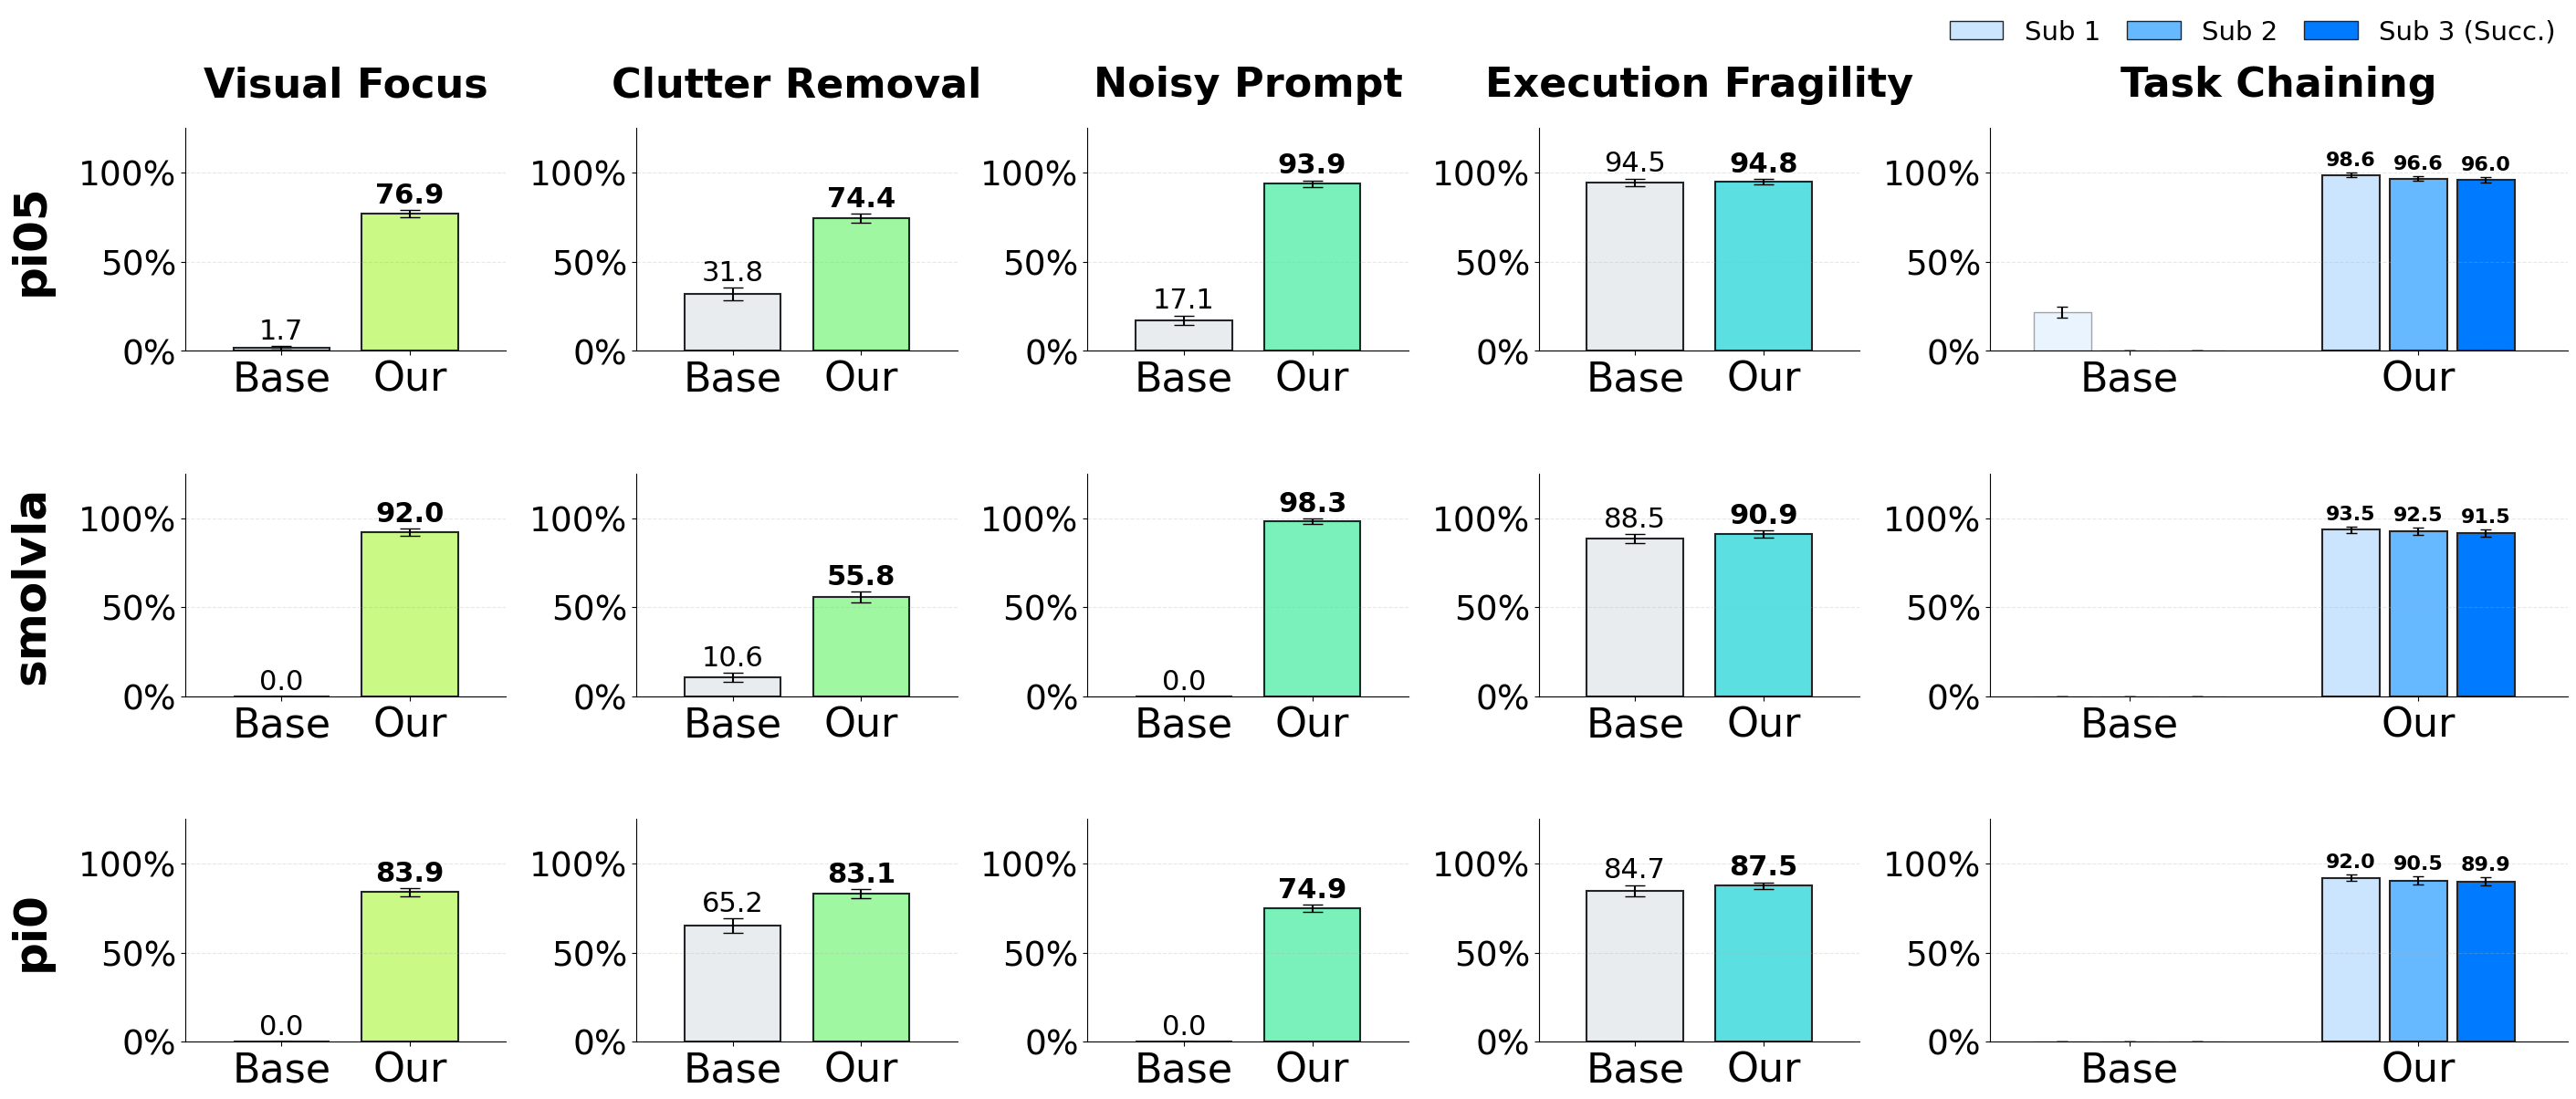
\includegraphics[width=\linewidth]{figure/result.png}
    \captionof{figure}{\textbf{LIBERO-\sys\ 上的性能。}比较 \sys\ 与 VLA 基线在视觉、语言和长时程挑战上的表现。}
    \label{fig:result}
  \end{minipage}%
  \hspace{0.01\textwidth}%
  \begin{minipage}[t]{0.30\textwidth}
    \vspace{0pt}
    \centering
    {\color{black}
    \vspace{0pt}
    \small
    \setlength{\tabcolsep}{3pt}
    \renewcommand{\arraystretch}{1.02}
    \begin{tabular}{@{}p{0.48\linewidth}lr@{}}
    \toprule
    \multicolumn{1}{@{}l}{\textbf{组件}} & & \textbf{ms/步} \\
    \midrule
    \multirow{2}{=}{基线 rollout} & 均值 & 15.31 \\
    & P95 & 15.98 \\
    \cmidrule(lr){1-3}
    \multirow{2}{=}{RAG 检索} & 均值 & 0.005 \\
    & P95 & 0.005 \\
    \cmidrule(lr){1-3}
    \multirow{2}{=}{VLM 编排} & 均值 & 7.20 \\
    & P95 & 8.65 \\
    \cmidrule(lr){1-3}
    \multirow{2}{=}{SAM3 + 叠加} & 均值 & 0.16 \\
    & P95 & 0.16 \\
    \cmidrule(lr){1-3}
    \multirow{2}{=}{SAM3 + 移除} & 均值 & 0.16 \\
    & P95 & 0.16 \\
    \bottomrule
    \end{tabular}
    \vspace{-0.3em}
    \captionsetup{justification=raggedright,singlelinecheck=false}
    \vspace{0.2em}
    \captionof{table}{\textbf{运行时开销。}在 1000 个 LIBERO 步上摊销。}
    \label{tab:runtime_overhead}
    \renewcommand{\arraystretch}{1.0}
    }
  \end{minipage}
  \vspace{-0.5em}
\end{figure*}

\begin{table}[t]
  \centering
  \caption{\textbf{LIBERO-PRO 上的性能。}布局（Pos）和语义（Task）偏移下的成功率。}
  \label{tab:libero_pro}
  \small
  \addtolength{\tabcolsep}{-4pt}
  {
  \setlength{\aboverulesep}{0pt}
  \setlength{\belowrulesep}{0pt}
  \begin{tabular}{l|clcc}
    \toprule
    \rule{0pt}{3ex} \textbf{层级} & \textbf{类别} & \textbf{任务（符号形式）} & \textbf{$\pi_{0.5}$基线} & \textbf{使用本文方法} \\
    \midrule
    \rule{0pt}{2.5ex} \multirow{6}{*}{\textbf{Pos}} & \multirow{5}{*}{\textbf{空间}}
      & $P.(btw(p, r), pl.)$         & 2\%  & \textbf{63.0\%} \\
    & & $P.(center, pl.)$             & 0\%  & \textbf{97.0\%} \\
    & & $P.(drw_{top}(cab_{w}), pl.)$ & 0\%  & \textbf{20.2\%} \\
    & & $P.(next\_to(p), pl.)$        & 0\%  & \textbf{57.0\%} \\
    & & $P.(next\_to(r), pl.)$        & 12\% & \textbf{71.0\%} \\
    \cmidrule(l){2-5}
    & \rule{0pt}{2.5ex} \textbf{物体} & $P.(soup, bskt.)$ & 0\% & \textbf{35.0\%} \\
    \midrule
    \multicolumn{3}{l|}{\rule{0pt}{2.5ex} \textit{\textbf{平均值（Pos）}}} & 2.33\% & \textbf{57.2\%} \\
    \midrule
    \rule{0pt}{3ex} \multirow{14}{*}{\textbf{Task}} & \multirow{9}{*}{\textbf{空间}}
      & $P.(btw(p, r), pl.)$       & 0\% & \textbf{78.0\%} \\
    & & $P.(center, pl.)$           & 2\% & \textbf{82.0\%} \\
    & & $P.(next\_to(ck.), pl.)$    & 2\% & \textbf{97.0\%} \\
    & & $P.(next\_to(p), pl.)$     & 0\% & \textbf{73.0\%} \\
    & & $P.(next\_to(r), pl.)$     & 2\% & \textbf{98.0\%} \\
    & & $P.(on(ck.), pl.)$          & 0\% & \textbf{12.0\%} \\
    & & $P.(on(r), pl.)$            & 2\% & \textbf{100.0\%} \\
    & & $P.(on(stove), pl.)$        & 0\% & \textbf{13.0\%} \\
    & & $P.(on(cab_{w}), pl.)$      & 0\% & \textbf{95.0\%} \\
    \cmidrule(l){2-5}
    & \rule{0pt}{2.5ex} \multirow{5}{*}{\textbf{物体}}
      & $P.(soup, bskt.)$           & 0\% & \textbf{16.0\%} \\
    & & $P.(bbq, bskt.)$            & 2\% & \textbf{32.0\%} \\
    & & $P.(juice, bskt.)$          & 2\% & \textbf{41.0\%} \\
    & & $P.(dressing, bskt.)$       & 0\% & \textbf{13.0\%} \\
    & & $P.(tomato, bskt.)$         & 0\% & \textbf{23.0\%} \\
    \midrule
    \multicolumn{3}{l|}{\rule{0pt}{2.5ex} \textit{\textbf{平均值（Task）}}} & 0.86\% & \textbf{55.2\%} \\
    \bottomrule
  \end{tabular}
  }
  \vspace{-1.5em}
\end{table}

我们在 25 项任务上，使用多个基础模型评估 \sys，并进一步通过消融实验验证双阶段记忆巩固机制。
结果表明，\sys\ 在不同场景下均能持续改善上下文内自适应和策略鲁棒性。

为在真实机器人实验成本和试验次数约束下提高统计可靠性，我们优先在高保真仿真环境中进行严格测试。

\subsection{实验设置}

\noindent\textbf{任务设计与评估基准。}
为评估分布偏移下的鲁棒上下文内自适应，我们在两个任务套件上进行实验。
首先采用 \textbf{LIBERO-PRO}~\cite{liberopro} 基准，测试空间和物体类别中位置交换（LIBERO-PRO Pos）与任务级变化（LIBERO-PRO Task）下的鲁棒性。

此外，我们提出 \textbf{LIBERO-\sys}。
该套件在仿真和真实机器人场景中形式化了五类\textit{常见且关键}的 OOD 挑战维度。
它通过重新配置 LIBERO 场景~\cite{libero_ref}中的资产，提供一个受控环境，用于评估智能体无需任务特定微调、针对反复出现的失败模式触发自适应干预的能力。

\begin{itemize}
    \item \textbf{视觉聚焦：}从五个外观相同的新碗中选择目标。我们用不可区分的资产替换 \textit{LIBERO-Spatial} 目标，以评估细粒度视觉歧义下的\textbf{指称落地}。

    \item \textbf{杂物移除：}在密集干扰物中抓取目标。我们在 \textit{LIBERO-Spatial} 中加入高熵物体簇，以测试拥挤场景中的\textbf{操作聚焦}和干扰缓解能力。

    \item \textbf{噪声提示：}从措辞或任务结构偏离历史成功经验模式的指令中提取意图（例如“呃……拿那个红色、捏起来软软的东西”）。我们向 \textit{LIBERO-Object} 指令注入语言噪声，以评估\textbf{语言鲁棒性}和\textbf{以经验为落地依据的语义映射}。

    \item \textbf{执行脆弱性：}细微滑动便会导致失败的关键操作。我们从 \textit{LIBERO-Object} 中整理不稳定子任务，以评估面对机械不确定性时的\textbf{操作稳定性}。

    \item \textbf{任务串联：}将多个物体分拣到篮子中的长时程任务。该任务通过串联原子的 \textit{LIBERO-Object} 动作，评估顺序工作流中的\textbf{长期推理}和\textbf{错误韧性}。
\end{itemize}

\noindent\textbf{上下文内初始化与指标。}
我们首先在标准 LIBERO-Object 和 LIBERO-Spatial 集上执行一次初步推理，以初始化双记忆 RAG。
这种非参数“冷启动”会用通用执行轨迹填充记忆库，但不进行基于梯度的训练，也不会接触评估时的 OOD 扰动。
随后，我们对每项任务运行 199 次随机化 rollout，充分打乱物体位姿和任务序列以减少偏差。
性能以\textbf{总体完成率}和\textbf{中间成功率}衡量，后者用于细粒度分析长时程任务。

\noindent\textbf{基线。}
我们在多种基础模型上评估 \sys，包括 $\pi_0$~\cite{pi0}、$\pi_{0.5}$~\cite{pi05} 和 SmolVLA~\cite{SmolVLA}。
在各 OOD 场景中，\sys\ 均持续提高成功率，表明策略泛化能力得到改善。

\subsection{主要结果}
\label{Main Results}

如图~\ref{fig:result} 和表~\ref{tab:libero_pro} 所示，\sys\ 增强的策略在 LIBERO-\sys\ 与 LIBERO-PRO 上均提高了鲁棒性，尤其是在感知歧义、语言噪声和长时程误差复合的情况下。

\subsubsection{LIBERO-\sys\ 上的结果}

\noindent\textbf{环境与语言变化。}
基础模型对感知和语言干扰十分敏感。
对于 \textit{pi05-LIBERO}，使用 \sys\ 后，\textit{视觉聚焦}和\textit{杂物移除}的成功率分别从 $1.7\%$ 和 $31.8\%$ 提升至 $76.9\%$ 和 $74.4\%$，说明基于 MCP 的干预有助于隔离与任务相关的物体。
对于语言扰动，\textit{smolvla-LIBERO} 经指令改写后在\textit{噪声提示}上的成功率达到 $98.3\%$。

\noindent\textbf{执行稳定性与长时程任务。}
在\textit{执行脆弱性}任务中，\sys\ 通过加入面向恢复的干预，使所有模型的成功率都提高到 $87\%$ 以上。
由于\textit{执行脆弱性}的基线成功率本来就相对较高，\sys\ 的绝对提升较小，主要通过回滚和重试减少剩余的少数失败。
在\textit{任务串联}中，\sys\ 通过子任务分解与控制流重置减少复合误差；值得注意的是，\textit{pi05-LIBERO} 到最后一个子任务仍保持 $96.0\%$ 的成功率。

\subsubsection{LIBERO-PRO 上的结果}

\noindent\textbf{位置级布局偏移。}
在 LIBERO-PRO Pos 下，$\pi_{0.5}$ 基线平均成功率仅为 $2.33\%$，而 \sys\ 将其提高到 $57.2\%$。
这表明记忆引导的视觉干预有助于在布局偏移下恢复物体落地。

\noindent\textbf{任务级语义扰动。}
在 LIBERO-PRO Task 下，基线平均成功率仅为 $0.86\%$，而 \sys\ 达到 $55.2\%$。
这些提升说明 \sys\ 改善了冻结控制器的输入和任务上下文，而不是替代底层 VLA 策略。

\subsubsection{讨论}
这些大幅提升源于对冻结 VLA 在 OOD 布局、干扰物、噪声提示和长时程链中无状态特性的补偿。
\sys\ 检索成功/失败记忆以诊断失败，并在执行前触发任务级 MCP 干预。

\subsubsection{在线延迟}
表~\ref{tab:runtime_overhead} 报告了在一个 1000 步 LIBERO 任务上摊销的延迟，其中基线 rollout 在 RTX 4090 上测得。
RAG 检索和基于 SAM3 的工具只增加可忽略的摊销开销，VLM 编排则是主要的额外成本。
由于 \sys\ 在 rollout 之前、而非每个策略步都调用这些模块，底层执行仍然流畅且非阻塞。
在流水线化的多任务设置中，下一项任务的编排可以与当前任务的执行重叠。

\subsection{消融实验}

在第~\ref{Main Results} 节验证编排器与 MCP 模块之后，我们进一步分析双记忆 RAG 系统的\textbf{双重}设计。
我们分两步进行：先分离双记忆库对执行效率的影响，再评估双阶段记忆巩固对推理深度的贡献。

\subsubsection{双记忆库的有效性}
\label{dual memory ablation}

为验证成功与失败经验在锚定编排器决策时都不可或缺，我们采用平均成功轮数（Average Turns-to-Success）~\cite{multiwoz,toolsandbox}，即达到最优方案所需的推理--干预循环次数。
当一次干预失败时，智能体会得到稀疏的环境反馈，并必须在后续轮次中自我纠正。
如图~\ref{fig:ablation_beeswarm} 所示，我们比较四种记忆配置：\textbf{无记忆}、\textbf{仅失败}、\textbf{仅成功}以及\textbf{\sys（双记忆）}。

\begin{figure}[htbp]
   \vspace{0.5em}
    \centering
    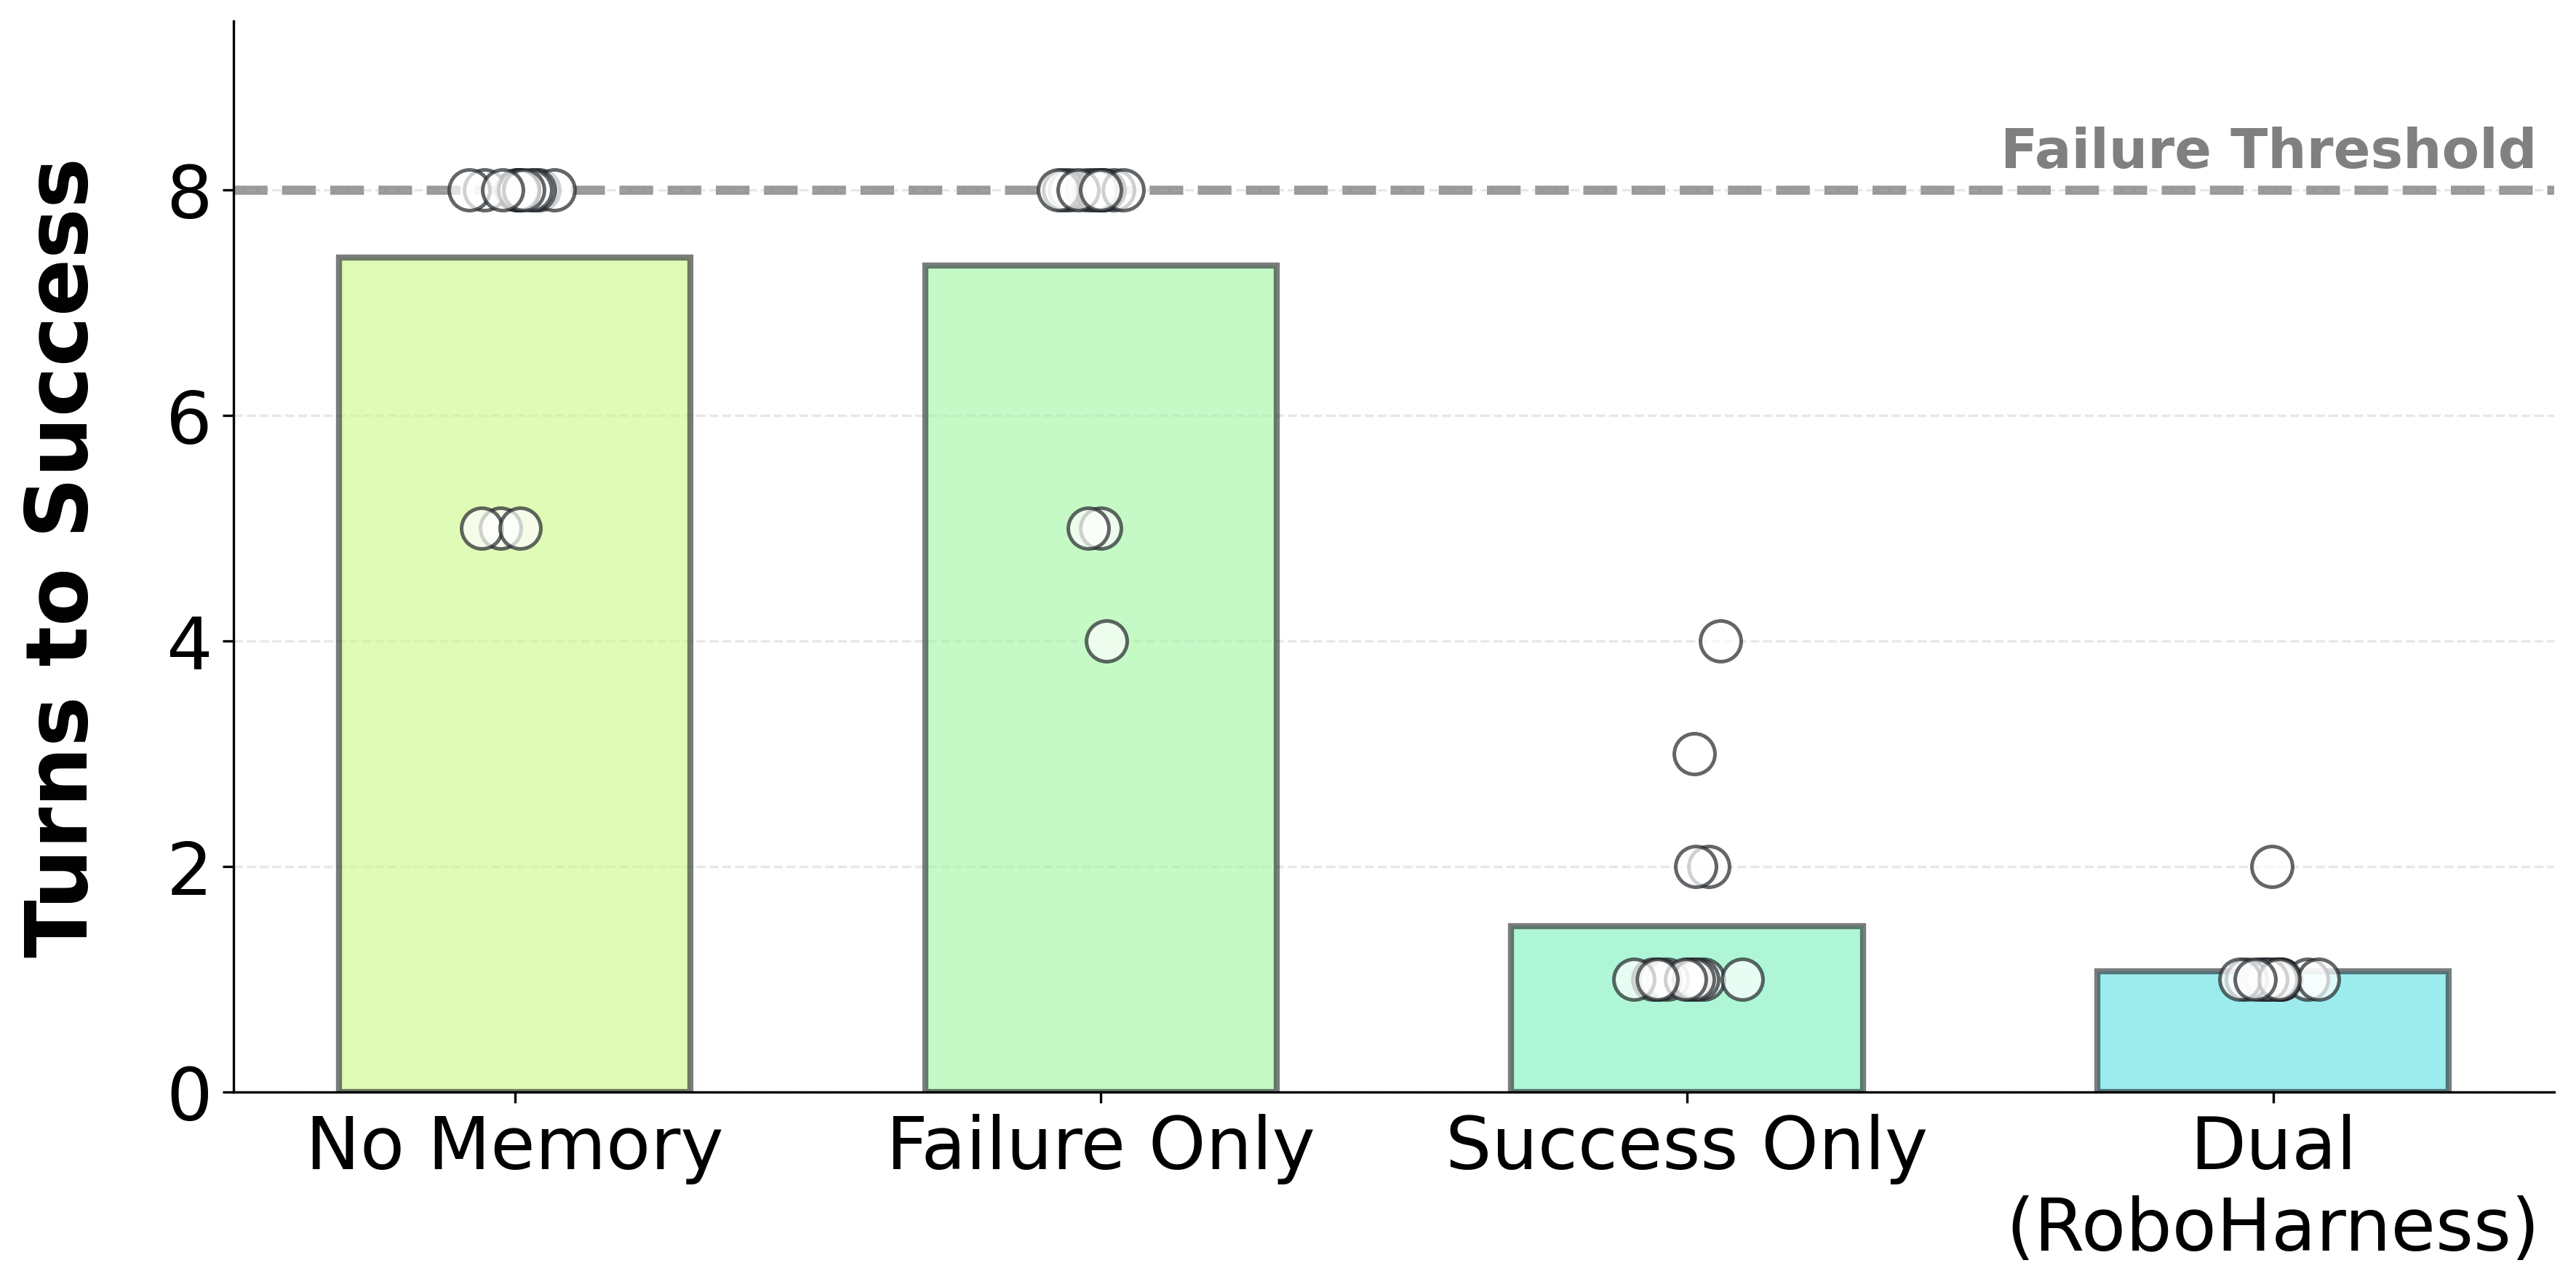
\includegraphics[width=0.4\textwidth]{figure/ablation_dual_memory.png}
    \caption{\textbf{消融实验。}达到目标干预方案所需推理轮数的分布。}
    \label{fig:ablation_beeswarm}
    \vspace{-0.5em}
\end{figure}

如图~\ref{fig:ablation_beeswarm} 所示，无记忆基线始终达到最大执行超时（$Mean=7.40$），表明零样本推理不足以实现 OOD 恢复。
虽然\textit{仅成功}记忆把平均轮数降至 $1.47$，但仍表现出显著的随机方差。
相比之下，\textbf{\sys（双记忆）}收敛到接近最优的\textbf{$1.07$} 轮。
双记忆库约束了视觉--语言编排器的搜索空间，使其能够进行有方向的决策，而非随机探索。

\subsubsection{双阶段记忆巩固的影响}

双记忆库提供原始数据，而这些经验的质量由第~\ref{Evolution} 节所述的迭代归因模块控制。
我们通过三种配置评估这一过程：\textbf{无 RAG}（基线）、\textbf{有限 RAG}（单阶段在线归因）以及\textbf{丰富 RAG}（\sys\ 的双阶段巩固）。

\newcolumntype{M}[1]{>{\centering\arraybackslash}m{#1}}
\renewcommand{\arraystretch}{1.1}
\setlength{\tabcolsep}{3pt}

\begin{table*}[t]
\vspace{0.5em}
\centering
\caption{\textbf{消融实验。}不同 RAG 配置的推理逻辑与成功率比较。}
\label{ablation}
\footnotesize
\begin{tabularx}{\textwidth}{|M{1.8cm}|X|M{3.5cm}|M{2.1cm}|M{1.8cm}|M{1.1cm}|}
\hline
\textbf{RAG 配置} & \multicolumn{1}{c|}{\textbf{通过 RAG 进行的编排器推理}} & \textbf{MCP 工具} & \textbf{动作结果} & \textbf{任务图像} & \textbf{SR（\%）} \\ \hline
\multirow{3}{*}{无 RAG} & 相同纹理导致目标身份存在歧义。 & $o_t' = \text{Paint-to-Action}(o_t, \theta_{\text{dist}})$ & 高亮碗 & \multirow{3}{*}{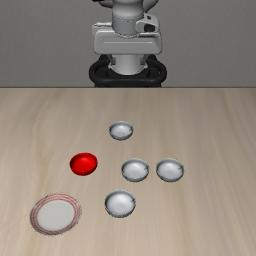
\includegraphics[width=0.95cm, valign=m]{figure/no_origin.jpg}} & \multirow{3}{*}{19.2} \\ \cline{2-4}
 & 盘子阴影可能造成检测错误。 & \texttt{none} & --- & & \\ \cline{2-4}
 & 背景干净，未发现干扰物。 & \texttt{none} & --- & & \\ \hline
\multirow{4}{*}{有限 RAG} & 靠近边缘造成遮挡；高亮目标。 & $o_t' = \text{Paint-to-Action}(o_t, \theta_{\text{dist}})$ & 高亮碗 & \multirow{4}{*}{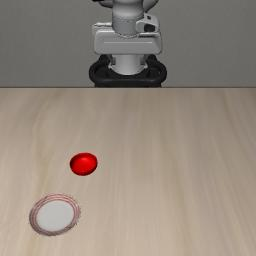
\includegraphics[width=0.95cm, valign=m]{figure/limit_origin.jpg}} & \multirow{4}{*}{48.8} \\ \cline{2-4}
 & 1. \textbf{过往失败}表明误识别风险较高。 & \multirow{2}{*}{$o_t'' = \text{Eraser}(o_t', \theta_{\text{conf}})$} & \multirow{2}{*}{移除 4 个干扰物} & & \\
 & 2. 通过\textbf{移除}相同干扰物来聚焦。 & & & & \\ \cline{2-4}
 & \textbf{替换背景}以减少视觉噪声。 & $o_t''' = \text{Eraser}(o_t'', \theta_{\text{conf}})$ & 替换背景 & & \\ \hline
\multirow{5}{*}{丰富 RAG} & 1. \textbf{失败记忆表明干扰物风险很高}。 & \multirow{4}{*}{$o_t' = \text{Eraser}(o_t, \theta_{\text{conf}})$} & \multirow{4}{*}{移除 4 个干扰物} & \multirow{5}{*}{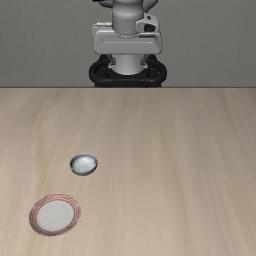
\includegraphics[width=0.95cm, valign=m]{figure/rich_origin.jpg}} & \multirow{5}{*}{60.1} \\
 & 2. \textbf{记忆}要求明确移除每一个碗。 & & & & \\
 & 3. 策略性保留目标和盘子。 & & & & \\
 & 4. 使用精确位置指导策略。 & & & & \\ \cline{2-4}
 & \textbf{已无干扰；无需视觉叠加。} & \texttt{none} & --- & & \\ \hline
\end{tabularx}
\end{table*}

\begin{figure}[htbp]
     \centering
     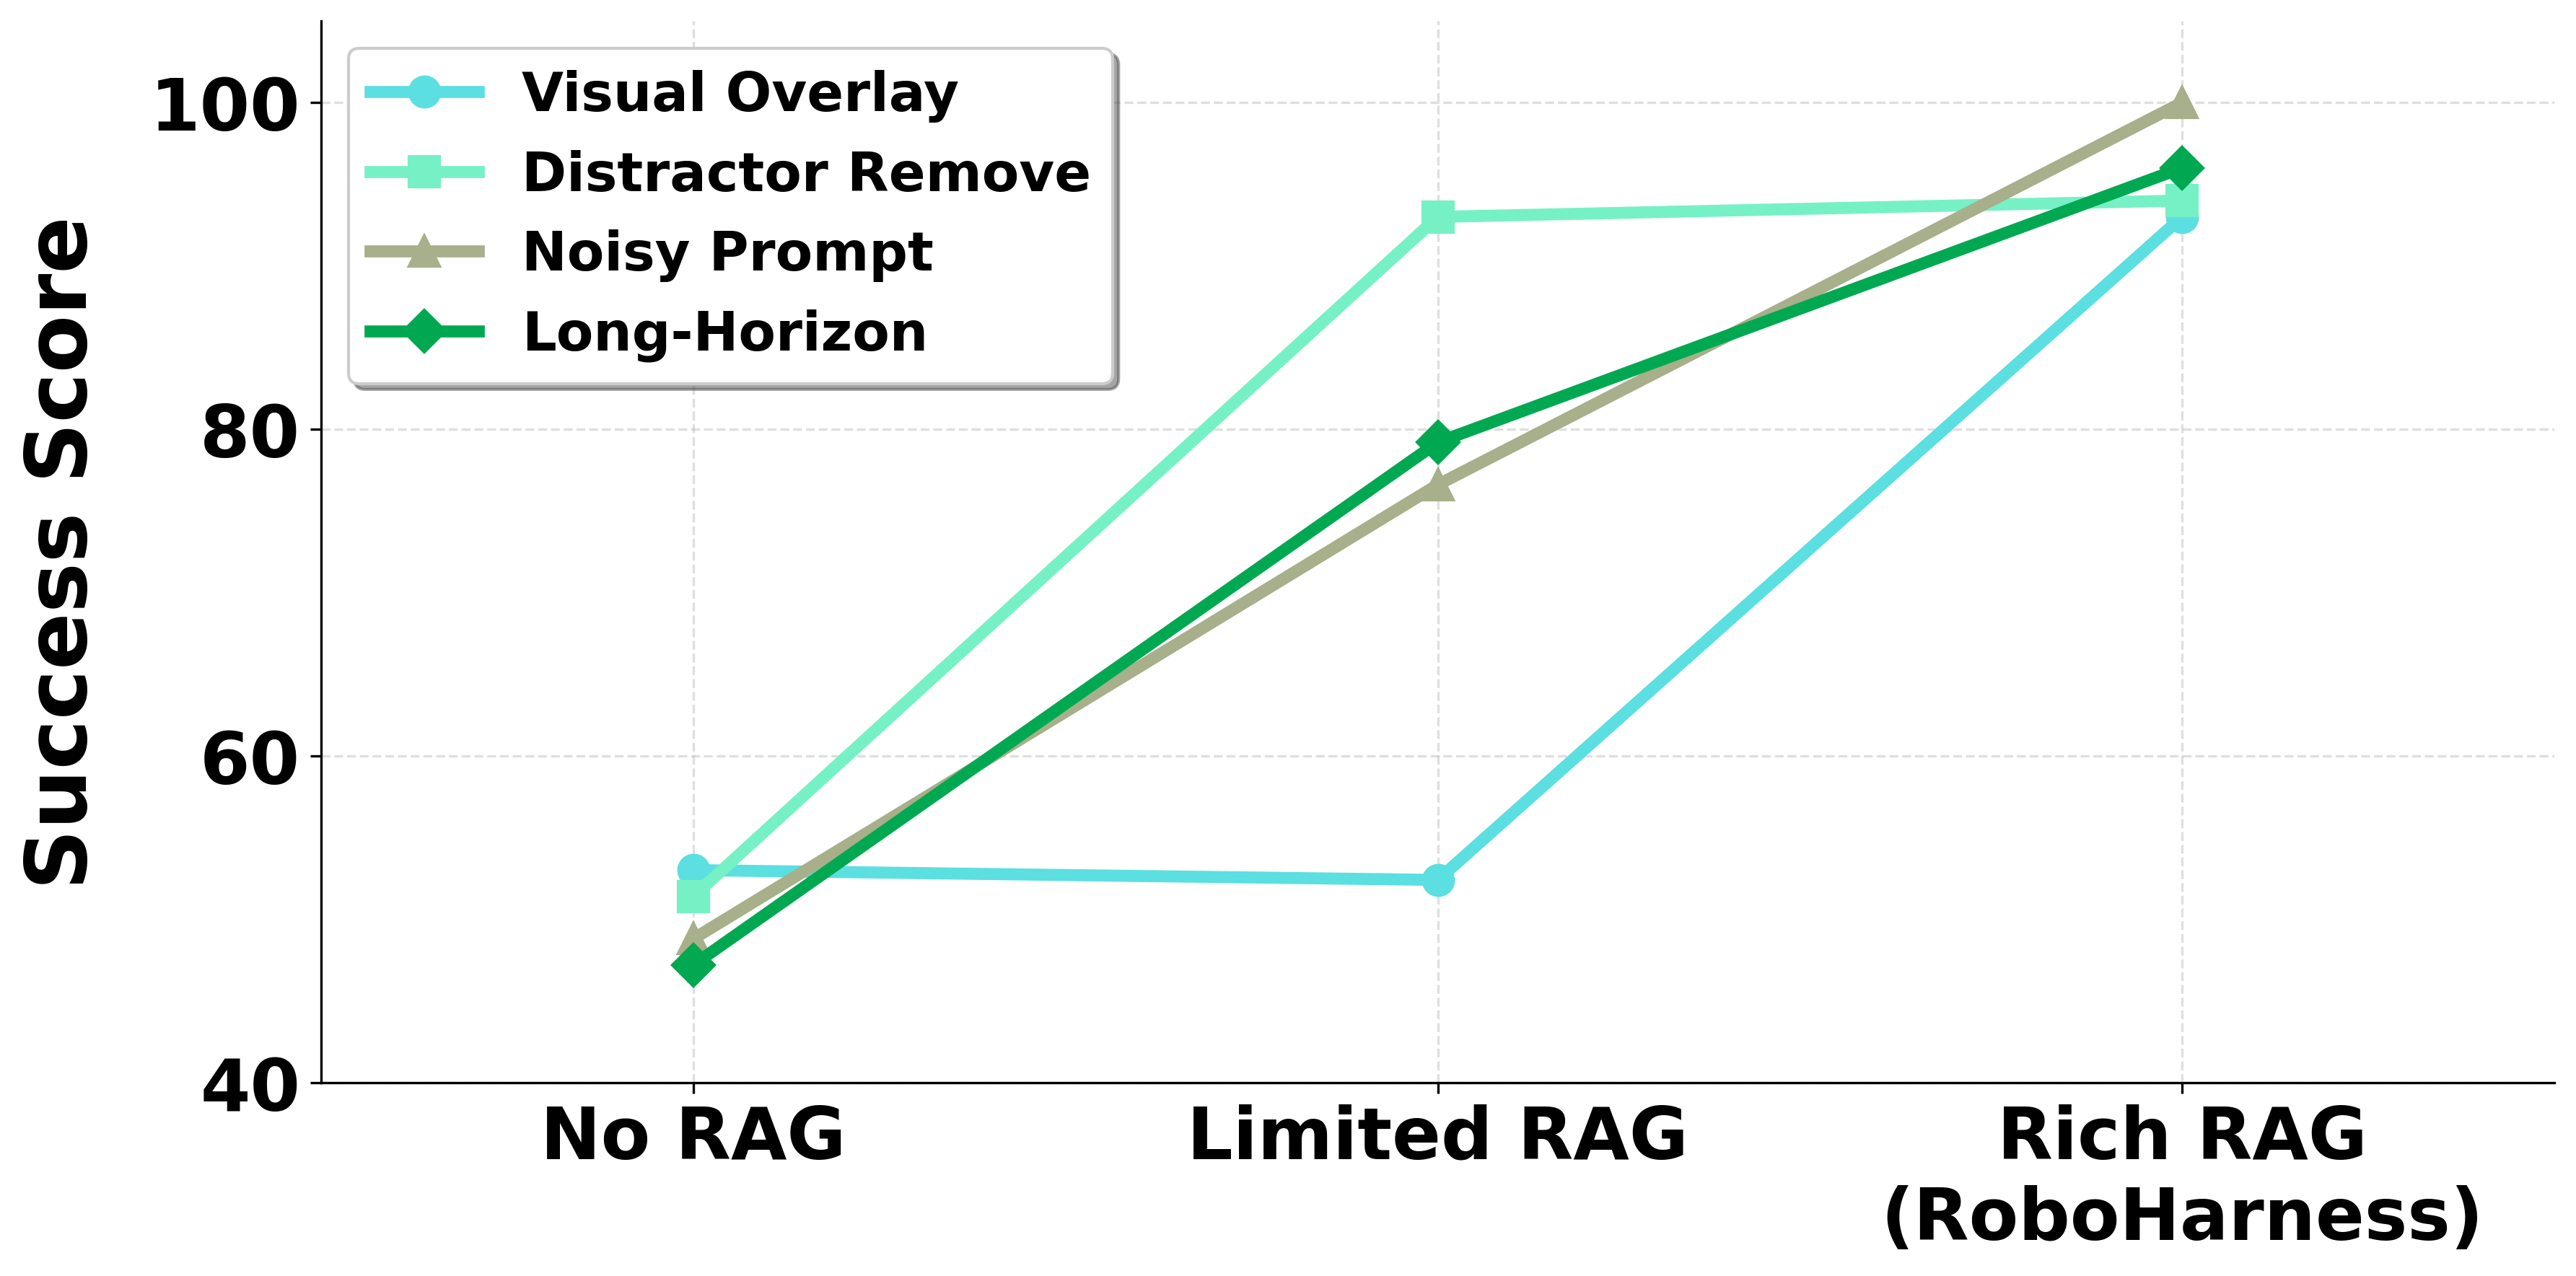
\includegraphics[width=0.4\textwidth]{figure/ablation2.png}
     \caption{\textbf{消融实验。}不同配置下定性推理深度分数的演化。}
     \label{score_qwen}
\end{figure}

\noindent\textbf{推理深度的定性评估。}
我们使用 Qwen3-VL-32B 为所生成指令的逻辑连贯性评分。
如图~\ref{score_qwen} 所示，丰富 RAG 在所有维度上始终取得最高评分。
这一提升来自更聚焦的推理轨迹：它们优先考虑关键干预点并减少无效动作。
这些结果表明，更高质量的 RAG 数据能改善因果理解，形成更鲁棒的工具调用链，与定量提升相一致。

\noindent\textbf{定量性能与稳定性。}
我们使用 $\pi_{0.5}$ 评估一个“杂物移除”变体。
如表~\ref{ablation} 所示，成功率随 RAG 信息丰富度提高。
无 RAG 的成功率仅为 $19.20\%$；与第~\ref{Main Results} 节比较可见，没有 RAG 的编排器指导会因引入负面偏差而适得其反。
有限 RAG 将性能提高到 $48.80\%$，但仍依赖冗余步骤（例如不必要的背景替换）。
丰富 RAG（\sys）使用精简的推理链达到 $60.10\%$，展现出更高的策略效率和精度。

\endinput

\section{结论}

在所测试的 OOD 场景中，许多 VLA 失败表现为感知、语言或协调局限，而不只是运动能力不足。
为解决这一问题，我们提出 \sys：一种记忆增强策略外壳。它通过动态 MCP 工具编排以及由检索、归因驱动推理和双阶段记忆巩固组成的闭环来包裹冻结的 VLA 策略，无需进行任何参数微调。
在多个 VLA 骨干模型上的评估表明，\sys\ 在多种 OOD 条件下都能持续改善上下文内自适应和鲁棒性。
未来工作将扩展 MCP 工具库以覆盖更广泛的失败模式，研究前沿多模态模型以进一步细化失败归因粒度，并探索这类记忆引导的干预如何迁移到更多样的真实机器人平台。

\section*{致谢}

我们衷心感谢匿名审稿人；他们的评审意见、反馈和建议显著改进了本工作。
本工作部分受到上海市科学技术委员会新一代信息技术项目（编号 25511104100）、国家自然科学基金（编号 62432010）以及教育部基础学科和交叉学科突破计划（JYB2025XDXM122）支持。
本工作还受到 OpenHarmony 具身智能项目管理委员会（PMC）支持。

\endinput


\bibliographystyle{IEEEtran}
\bibliography{ref}

\end{document}
